

%%*************************************************************************
%% Legal Notice:
%% This code is offered as-is without any warranty either expressed or
%% implied; without even the implied warranty of MERCHANTABILITY or
%% FITNESS FOR A PARTICULAR PURPOSE! 
%% User assumes all risk.
%% In no event shall the IEEE or any contributor to this code be liable for
%% any damages or losses, including, but not limited to, incidental,
%% consequential, or any other damages, resulting from the use or misuse
%% of any information contained here.
%%
%% All comments are the opinions of their respective authors and are not
%% necessarily endorsed by the IEEE.
%%
%% This work is distributed under the LaTeX Project Public License (LPPL)
%% ( http://www.latex-project.org/ ) version 1.3, and may be freely used,
%% distributed and modified. A copy of the LPPL, version 1.3, is included
%% in the base LaTeX documentation of all distributions of LaTeX released
%% 2003/12/01 or later.
%% Retain all contribution notices and credits.
%% ** Modified files should be clearly indicated as such, including  **
%% ** renaming them and changing author support contact information. **
%%*************************************************************************






\documentclass[compsoc,10pt]{IEEEtran}
% Some/most Computer Society conferences require the compsoc mode option,
% but others may want the standard conference format. 
\usepackage[labelfont=bf,textfont={bf}]{caption}

%\usepackage{cite}
\newcommand{\IT}{\sffamily{SNEAK}}
\usepackage{dblfloatfix}
\usepackage{tabularx}
\usepackage{booktabs}
\usepackage[numbers]{natbib}
\usepackage{amsmath}
\usepackage{url}
\usepackage{colortbl}
\usepackage[table]{xcolor}
\usepackage{rotating}
\usepackage{amssymb}
\usepackage{blindtext}
\usepackage{wrapfig}
\usepackage{graphicx}
\usepackage{csvsimple}
\usepackage{algorithm}
\usepackage[noend]{algpseudocode}
\usepackage{float}
\usepackage{aliascnt}
\usepackage{multirow}
\usepackage{soul}
\usepackage{color, colortbl}
\usepackage{babel,adjustbox,booktabs,multirow}
\usepackage[most]{tcolorbox}
\usepackage{subcaption}
\usepackage{balance}
\usepackage{pifont}
\usepackage{changepage}
\usepackage{framed}

\newcommand{\tick}{\ding{51}}
\newcolumntype{L}{>{\raggedright\arraybackslash}X}

\algnewcommand\algorithmicforeach{\textbf{foreach}}
\algdef{S}[FOR]{ForEach}[1]{\algorithmicforeach\ #1\ \algorithmicdo}

\newaliascnt{eqfloat}{equation}
\newfloat{eqfloat}{h}{eqflts}
\floatname{eqfloat}{Equation}

\newtcolorbox{myquote}{colback=lightgray!20!white,colframe=yellow!75!black,grow to right by=-10mm,grow to left by=-10mm,
    boxrule=0pt,boxsep=0pt,breakable} \makeatletter

\newcommand{\blockquote}[1]{  \begin{myquote}  #1  \end{myquote}  }


\newcommand*{\ORGeqfloat}{}
\let\ORGeqfloat\eqfloat
\def\eqfloat{%
  \let\ORIGINALcaption\caption
  \def\caption{%
    \addtocounter{equation}{-1}%
    \ORIGINALcaption
  }%
  \ORGeqfloat
}

\makeatletter
\renewenvironment{framed}{%
 \def\FrameCommand##1{\hskip\@totalleftmargin
 \fboxsep=\FrameSep\fbox{##1}
     \hskip-\linewidth \hskip-\@totalleftmargin \hskip\columnwidth}%
 \MakeFramed {\advance\hsize-\width
   \@totalleftmargin\z@ \linewidth\hsize
   \@setminipage}}%
 {\par\unskip\endMakeFramed}
\makeatother

% environment derived from framed.sty: see leftbar environment definition
\definecolor{formalshade}{rgb}{0.93,0.93,0.93}
\newcommand{\gray}{\cellcolor{lightgray}}

\definecolor{darkblue}{rgb}{0.2, 0.2, 0.2}

\newenvironment{formal}{%
  \def\FrameCommand{%
    \hspace{1pt}%
    {\color{darkblue}\vrule width 2pt}%
    {\color{formalshade}\vrule width 4pt}%
    \colorbox{formalshade}%
  }%
  \MakeFramed{\advance\hsize-\width\FrameRestore}%
  \noindent\hspace{-1pt}% disable indenting first paragraph
  \begin{adjustwidth}{}{7pt}%
  \vspace{2pt}\vspace{2pt}%
}
{%
  \vspace{3pt}\end{adjustwidth}\endMakeFramed%
}

\newcommand{\rqn}[1]{\underline{\textbf{RQ#1:}}}

\newcommand{\quart}[4]{\begin{adjustbox}{max width=.1\textwidth}\begin{picture}(100,5)%1
    {\color{black}\put(#3,2){\circle*{7}}\put(#1,2){\line(1,0){#2}}}\end{picture}\end{adjustbox}}

\usepackage{enumitem}
\setlist{nosep} 
\newcommand{\bi}{\begin{itemize}}
	\newcommand{\ei}{\end{itemize}}
\newcommand{\be}{\noindent\begin{enumerate}}
	\newcommand{\ee}{\noindent\end{enumerate}}

\newcommand{\bluecheck}{}%
\DeclareRobustCommand{\bluecheck}{%
  \tikz\fill[scale=0.4, color=blue]
  (0,.35) -- (.25,0) -- (1,.7) -- (.25,.15) -- cycle;%
}

\usepackage[tikz]{bclogo}
\newenvironment{RQ}[1]%
{\noindent\begin{minipage}[c]{\linewidth}%
\begin{bclogo}[couleur=gray!20,%
                arrondi=0,logo=\none,% 
                ombre=true%
                ]{{\small  ~#1}}}%
{\end{bclogo}\vspace{2mm}\end{minipage}}

%% reviewing
\newcommand{\blue}[1]{{\color{blue}{#1}}}
\newcommand{\reponse}[1]{\noindent{#1\\}}
\newcommand{\todo}[1]{\textbf{\color{red}{#1}}}
\newcommand{\subsect}[1]{\SS\ref{subsect:#1}}

%% Response text prefix
\newcommand{\respto}[1]{
\fcolorbox{black}{black!15}{%
\label{resp:#1}%
\bf\scriptsize R{#1}}}

%% Response text prefix
\newcommand{\bareresp}[1]{
\fcolorbox{black}{black!15}{%
\bf\scriptsize R{#1}}}
\newcommand{\BLUE}{\color{blue}}
\newcommand{\BLACK}{\color{black}}
\newcommand{\ORANGE}{\color{orange}}

%% Cite responses
\newcommand{\citeresp}[1]{%
{(see }\fcolorbox{black}{black!15}{%
\bf\scriptsize R{#1}}~{{on page \pageref{resp:#1})}}}%

% Response environment
\newenvironment{response}[1]{
    \BLUE \respto{#1}
} {
    \BLACK
}

\newenvironment{draftresponse}[1]{
    \ORANGE \respto{#1}
} {
    \BLACK
}




\begin{document}

% paper title
% Titles are generally capitalized except for words such as a, an, and, as,
% at, but, by, for, in, nor, of, on, or, the, to and up, which are usually
% not capitalized unless they are the first or last word of the title.
% Linebreaks \\ can be used within to get better formatting as desired.
% Do not put math or special symbols in the title.
%\IEEEspecialpapernotice{(Invited Paper)}


\title{How to Find Actionable Static Analysis Warnings: A Case Study with FindBugs}


\author{Rahul Yedida, 
Hong Jin Kang,
Huy Tu, Xueqi Yang, David Lo~\IEEEmembership{Fellow,~IEEE}, 
        Tim~Menzies,~\IEEEmembership{Fellow,~IEEE}
\IEEEcompsocitemizethanks{\IEEEcompsocthanksitem R. Yedida, X. Yang and  T. Menzies are with the Department
of Computer Science, North Carolina State University, Raleigh, USA.
 \protect\\
E-mail: ryedida@ncsu.edu, xyang37@ncsu.edu, timm@ieee.org
\IEEEcompsocthanksitem H.J. Kang and D. Lo are with the School of Computing and Information Systems, Singapore Management University, Singapore.
\protect\\
E-mail: hjkang.2018@smu.edu.sg, davidlo@smu.edu.sg
\IEEEcompsocthanksitem  H. Tu is with Meta Platforms, Inc. 
E-mail: huyqtu7@gmail.com}}


% The paper headers
\markboth{IEEE Transactions on Software Engineering}%
{Yedida \MakeLowercase{\textit{et al.}}: How to Recognize and Avoid Static Code Analysis False Alarms}

% make the title area
\IEEEtitleabstractindextext{
\begin{abstract}
Automatically generated static
code warnings  suffer from
a large number of false alarms.
Hence, developers
only take action
on a small percent of those warnings. 
To better predict which  static code warnings
should {\em not} be ignored, 
  we suggest that      analysts
  need to look deeper
  into their algorithms to find choices
 that better improve the particulars of their specific problem. Specifically,
 we show here that effective predictors
 of such warnings can be created   by methods
that {\em locally adjust} the decision boundary
(between actionable warnings and others).
 These  methods yield a  new high water-mark for recognizing actionable static code warnings.
For eight open-source Java projects
(CASSANDRA, JMETER, COMMONS, LUCENE-SOLR,
ANT, TOMCAT, DERBY)
 we    achieve perfect test results on 4/8 datasets
 and, overall, a median AUC (area under the true negatives, true positives curve) of 92\%. 


% Our conclusions are two-fold.
 
% had many corruptions. In the 

% Data set used to train such tools suffer
% from 

% X Yang, J Chen, R Yedida, Z Yu, T Menzies


% X Yang, Z Yu, J Wang, T Menzies

% A recent work by \citet{yang2021learning} claimed that recognizing static code false alarms was an intrinsically easy problem, citing the low intrinsic dimensionality of the data. This study used SVMs to effectively predict actionable static code warnings. However, it was refuted by an ICSE '22 paper by \citet{kang2022detecting}, who detailed how the data used by the former study was incorrectly labeled and provided a new dataset with corrected labels. 

% In this paper, we revisit the problem using the new, corrected data. We show that like the study by \citet{yang2021learning}, the corrected data still has low intrinsic dimensionality. Moreover, classical ML models are still the best choice for predicting actionable static code warnings (median AUC = 1.0). However, manual labeling, as was done to rectify the dataset, remains an expensive task. Therefore, we explore the problem under the semi-supervised setting. In this setting, classical ML models are insufficient, leading us to turn to neural approaches for solving this task. In the spirit of testing simpler algorithms before more complex ones \cite{fu2017easy}, we first started with feedforward networks (also called artificial neural networks), using the GHOST framework proposed by \citet{yedida2021value}, which uses hyper-parameter optimization along with a ``fuzzy sampling'' technique to achieve state-of-the-art results in defect prediction. We augment the feedforward learner used by GHOST with a trivial semi-supervised learning approach. This yields new high water-mark results on the dataset (while using 9.5\% of the labels), achieving perfect test results on 4/8 datasets (median AUC = 0.92). We characterize this final approach, which we call ``GHOST2'', as a combination of several different engineering techniques.  Finally, we perform an ablation study that tests whether each component of GHOST2 is necessary, including testing deep learners (specifically, convolutional neural networks, and the CodeBERT \cite{feng2020codebert} system), which shows that all parts of GHOST2 are necessary (and that feedforward networks are sufficient) and contribute to its performance.

% Our contributions are many-fold: (a) we present a case study of a successful collaboration between authors of the \citet{yang2021learning} and \citet{kang2022detecting} studies (b) we show that even with the revised dataset, the problem is still intrinsically simple (c) we develop a novel system called ``GHOST2'' that achieves a new high water-mark in performance on the corrected data under the low label availability setup (d) we show a ``small data'' effect where neural approaches outperform other approaches on smaller datasets ($<30$ samples), a reversal of common belief (e) we characterize learning problems as a set of engineering techniques, each of which needs to be carefully attended to, rather than using tools off-the-shelf for each (f) we explain why fuzzy sampling helps optimization.
        

\end{abstract}



% Note that keywords are not normally used for peer review papers.
\begin{IEEEkeywords}
software analytics, static analysis; false alarms; locality,  hyperparameter optimization
\end{IEEEkeywords}}

\maketitle

% For peer review papers, you can put extra information on the cover
% page as needed:
% \ifCLASSOPTIONpeerreview
% \begin{center} \bfseries EDICS Category: 3-BBND \end{center}
% \fi
%
% For peer review papers, this IEEEtran command inserts a page break and
% creates the second title. It will be ignored for other modes.
\IEEEpeerreviewmaketitle

% xxxx from david: comfercing to fix refautions t commin


\section{Introduction}\label{intro}
  

Static analysis (SA) tools report errors
in source code, without needing to execute that code. This makes them very popular in industry. For example, the FindBugs tool~\cite{ayewah2010google}
%of Figure~\ref{fig:fb} 
has been downloaded over a million times. Unfortunately, due to the imprecision of static analysis and the different contexts where bugs appear, SA tools often suffer from
a large number of false alarms that are deemed to be not actionable~\cite{tomassi2021real}.
Hence, developers never act on most of 
their warnings \cite{heckman2008establishing, heckman2009model, kim2007warnings}. 
 Previous research work shows that   35\% to
91\% of SA warnings reported as bugs by SA tools 
are routinely
ignored by developers~\cite{heckman2009model,heckman2008establishing,kim07}.

Those  false alarms produced by SA tools are a significant barrier to the wide-scale adoption of these SA tools ~\cite{johnson2013don,ChristakisB16}. 
Accordingly, in 2018~\cite{wang2018there}, 2020~\cite{yang2021learning}
and 2021~\cite{yang2021understanding}, Wang et al. and Yang et al. proposed
data miners that  found the subset of static code warnings that
developers found ``actionable'' (i.e. those that
motivate developers to change the code). 
But in 2022, Kang et al.~\cite{kang2022detecting} showed that of the
31,000+ records used by  
Wang et al. and Yang et al., they could only generate 768  error-free records-- which meant all the prior Wang and Yang et al. results need to be revisited.

When Kang et al. tried to build predictors from the 768 good records, they found that their   best-performing predictors were not effective
(e.g., very low median AUCs of 41\%), for details see 
Table~\ref{tab:initial_svm}. 
  Hence the following remains an open research question:
 
 

\begin{formal}\noindent\rqn{1} \textit{For detecting actionable static code warnings,
what data mining methods should we recommend?}
\end{formal}
\noindent
This paper conjectures that prior work failed to find good predictors because of a {\em locality problem}. In the learners
used in that prior work, the decision boundary between  
between actionable warnings and other
was determined by a single {\em global policy}. 
\BLUE \respto{1a11.1} In detail, changes to the values of the hyper-parameters of the SVM learner that they employed make \textit{global} changes to the decision boundary (i.e., the global shape of the decision boundary is modified); instead, we argue for \textit{local} changes to the decision boundary. This allows us to make different local adjustments at different regions of the decision boundary to adapt it to the local data.
\BLACK
 
More specifically, we conjecture  that:
 \begin{quote}
 {\em 
 For complex data, \underline{\bf global} treatments  
   perform worse  than \underline{\bf localized} treatments
 which   adjust different parts of the  landscape in 
 different ways.}
 \end{quote}
 To test this, we use    {\em local} treatments to adjust the decision boundary
  in different ways in different parts of the data.
 \be
\item
{\em Boundary engineering}:  adjust the decision boundary near our data points;
\item
{\em Label engineering}:   control outliers
in a local region by using just a small fraction of those local labels;
\item
{\em Instance engineering}: addressing class imbalance in local regions of the data
\item
These treatments are combined with
{\em parameter engineering}  to control   how we   build models.
 \ee
We call this combination of   treatments
GHOST2 (GHOST2 extends GHOST~\cite{yedida2021value} which just used one of these treatments).  When researchers propose an intricate
combination of 
ideas, it is prudent to ask several questions:
   
\begin{formal}\noindent 
\rqn{2} {\em Does GHOST2's  combination of {\em instance}, {\em label}, {\em boundary}  and {\em parameter} engineering, reduce the complexity of  the decision boundary?}
\end{formal}

Later in this paper, we will show evidence that our proposed methods
simplifies the ``error landscape'' of a data set (a concept which we will discuss, in detail in \S\ref{rx}).

 
\begin{formal}\noindent 
\rqn{3} {\em Does  GHOST2's  use of {\em instance}, {\em label}, {\em boundary}  and {\em parameter} treatments improve predictions?} 
\end{formal}
  
 Using data from Kang et al. (768 records from  eight open-source Java projects), we show that
 GHOST2  was able to generate excellent predictors for actionable static code warnings.




\begin{figure*}[!t]
\begin{center}
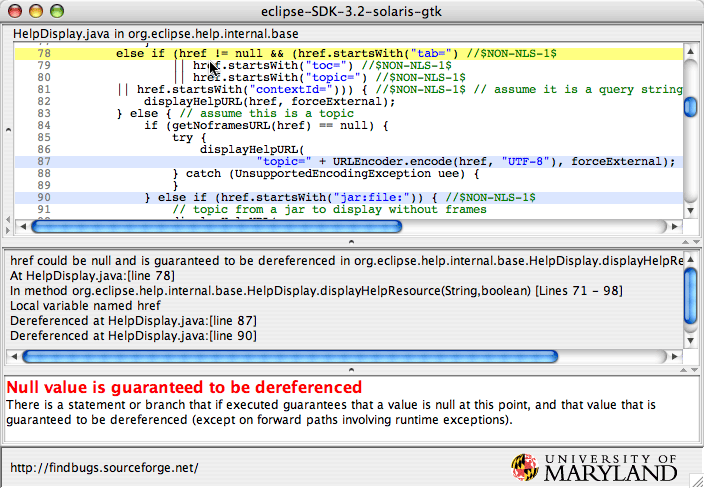
\includegraphics[width=3.8in]{tim/guaranteedDereference.png}\end{center}
\caption{Example of a static analysis warning, generated via the FindBugs
tool~\cite{ayewah2010google}.}\label{fig:fb}
\end{figure*}

%Given that GHOST2 has many parts, we should also ask:
 \begin{formal}\noindent   
\rqn{4} {\em Are all parts of GHOST2 necessary; i.e. would something
simpler also achieve the overall goal?}
\end{formal}

   
   To answer {\bf RQ4},   this paper   reports an 
{\em ablation study} that removes
one treatment at a time from our four recommended treatments. For the purposes of 
recognizing and avoiding
static code analysis false alarms, it will be shown that,
ignoring any part of our proposed solution   leads
to worse predictors.
Hence, while we do not know if  changes to our design might lead to {\em better}
predictors, the
ablations study does show that removing anything from that design makes matters {\em worse}.
 
   
This work has six key contributions:
\be
\item
As a way to address, in part, the methodological problems raised by Kang et al. GHOST2 makes its conclusions using   a small percentage of the raw data (10\%). That is, to address the issues
of corrupt data found by Kang et al., we say ``use less data'' and, for the data that is used,   ``reflect more on that data''.
\item
A case study of successful open collaboration
by software analytics researchers. 
This paper is joint work between the Yang et al. and Kang et al. teams
from the United States and Singapore. By recognizing a shared problem, then sharing  data and tools, in eight weeks these two teams produced a new
state-of-the-art result that improves on all of the past  
papers by these two teams (within this research arena). This illustrates the value of open and collaborative science, where groups with different initial findings come together to help each other in improving the state-of-the-art for the benefit of science and industry.
\item
Motivation for changing the way we train  software analytics newcomers.  It may not be enough to just reflect on the
different properties of off-the-shelf learners.
% Rather, future improvements in software analytics may require more than, e.g., just applying off-the-shelf deep learning. 
Analysts may need to be skilled in
boundary, label, parameter and instance engineering.
\item GHOST2's  design, implementation, and evaluation.
\item A new high-water mark in software analytics for learning actionable static code warnings.
\item A reproduction package  that other researchers can use to repeat/refute/improve on our results\footnote{ \url{https://github.com/yrahul3910/static-code-warnings/}}.


\ee
% Perhaps, in the future,
% instead of rushing to refute   each
% others' work, it might serve the goals
% of science and industry better if we rushed
% to collaborations with each  other to help
% % each other improve our work.
The rest of this paper is structured as follows. The next section offers some background notes. \S \ref{problem} discusses the locality
problem for complex data sets and \S \ref{rx}
offers details on our treatments.  \S \ref{sec:methods} describes our experimental methods
after which, in \S \ref{sec:results}, we show that GHOST2      outperforms (by a large margin) prior results from Kang et al. We discuss threats to validity for our study in \S \ref{sec:threats}, before a discussion in \S \ref{sec:discussion} and concluding in \S \ref{sec:conclusion}.

 


Before all that,  we digress to   stress the following:
\bi
\item
A  learned model must be tested on the kinds of data expected in practice. 
\item
Hence,  
  any treatments to the data  (e.g.  via instance, label, boundary engineering) 
  {\em are restricted to the training data, and do {\bf not} affect the test  data.}
\ei




% Science is meant to be about a community critiquing and improving each other's ideas. We offer here a successful example of such a community interaction where teams from Singapore and the US successfully worked together. Initially, the Singapore team refuted the results of the other in a high-profile ICSE’22 paper. Subsequently, the teams worked together to produce new results that clarified and improved the old work.
 
% We write to suggest that this kind of interaction should be routine, and not some rare exceptional case. As seen here, software analytics is not just the application of some turnkey off-the-shelf algorithm; rather, to improve on prior results it is necessary to perform an extensive excursion across a wide range of tools. As shown below, that excursion can take some strange paths. For example, below we improve on the prior state of the art using five methods which, according to the truisms of our field, should not have worked. Yet, they did suggest that SE data is very diverse, and successful analytics requires a wide range of applications– sometimes even using things that established wisdom says should not work.



% \hl{Add more stuff here}

 
 
\section{Background}
\label{sec:background}

\input{tim/science1}

 

\subsection{Static Code Analysis}
Automatic static analysis (SA) tools, such as Findbugs
%(see Figure~\ref{fig:fb}), 
are tools for   detecting bugs in source code,
without having to execute that code.
As they can find real bugs at low cost~\cite{thung2012extent,habib2018many}, they have been adopted in open source projects and in industry~\cite{ayewah2010google,sadowski2018lessons,beller2016analyzing,zampetti2017open,panichella2015would,vassallo2020developers}.
However, as they do not guarantee that all warnings are real bugs, 
these tools produce false alarms. 
The large number of false alarms produced is a barrier to adoption~\cite{johnson2013don,ChristakisB16}; it is easy to imagine how developers will be frustrated by using tools that require them to inspect numerous false alarms before finding a real bug.
While false alarms include spurious warnings caused by the over-approximation of possible program behaviors during program analysis, 
false alarms also refer to warnings that developers do not act on.
For example, developers may not think that the warning represents a bug (e.g. due to ``style'' warnings that developers perceive to be of little benefit) or may not wish to modify obsolete code. 

The problem of addressing false alarms from static analysis tools has been widely studied.
There have been many recent attempts to address the problem. 
Some researchers have proposed new SA tools that use  more sophisticated, but costly, static analysis techniques (e.g. Infer~\cite{calcagno2015moving}, NullAway~\cite{banerjee2019nullaway}).
Despite their improvements, these tools still produce many false alarms~\cite{tomassi2021real}.
Other attempts to prune false alarms include the use of test case generation to validate the presence of a bug  at the source code location indicated by the warning~\cite{kallingal2021validating}.
As generating test cases is expensive, these techniques may face issues when scaling up to larger projects, limiting their practicality.


\subsection{Early Results:  Wang et al., 2018}


By framing the problem as a binary classification problem, 
  machine learning techniques can identify actionable warnings 
  (allowing us to prune false alarms)~\cite{hanam2014finding,heckman2008establishing,liang2010automatic,ruthruff2008predicting,wang2018there,yang2021learning,yang2021understanding}.
These techniques use features extracted from code analysis and metrics computed over the code and warning's history in the project.
Figure \ref{fig:workflow} illustrates this process. 
A static analyzer is ran on a training revision and the warnings produced are labelled. 
When applied to the latest revision, only warnings classified as actionable warnings by the machine learner are presented to the developers.

\begin{figure}[t]
  
  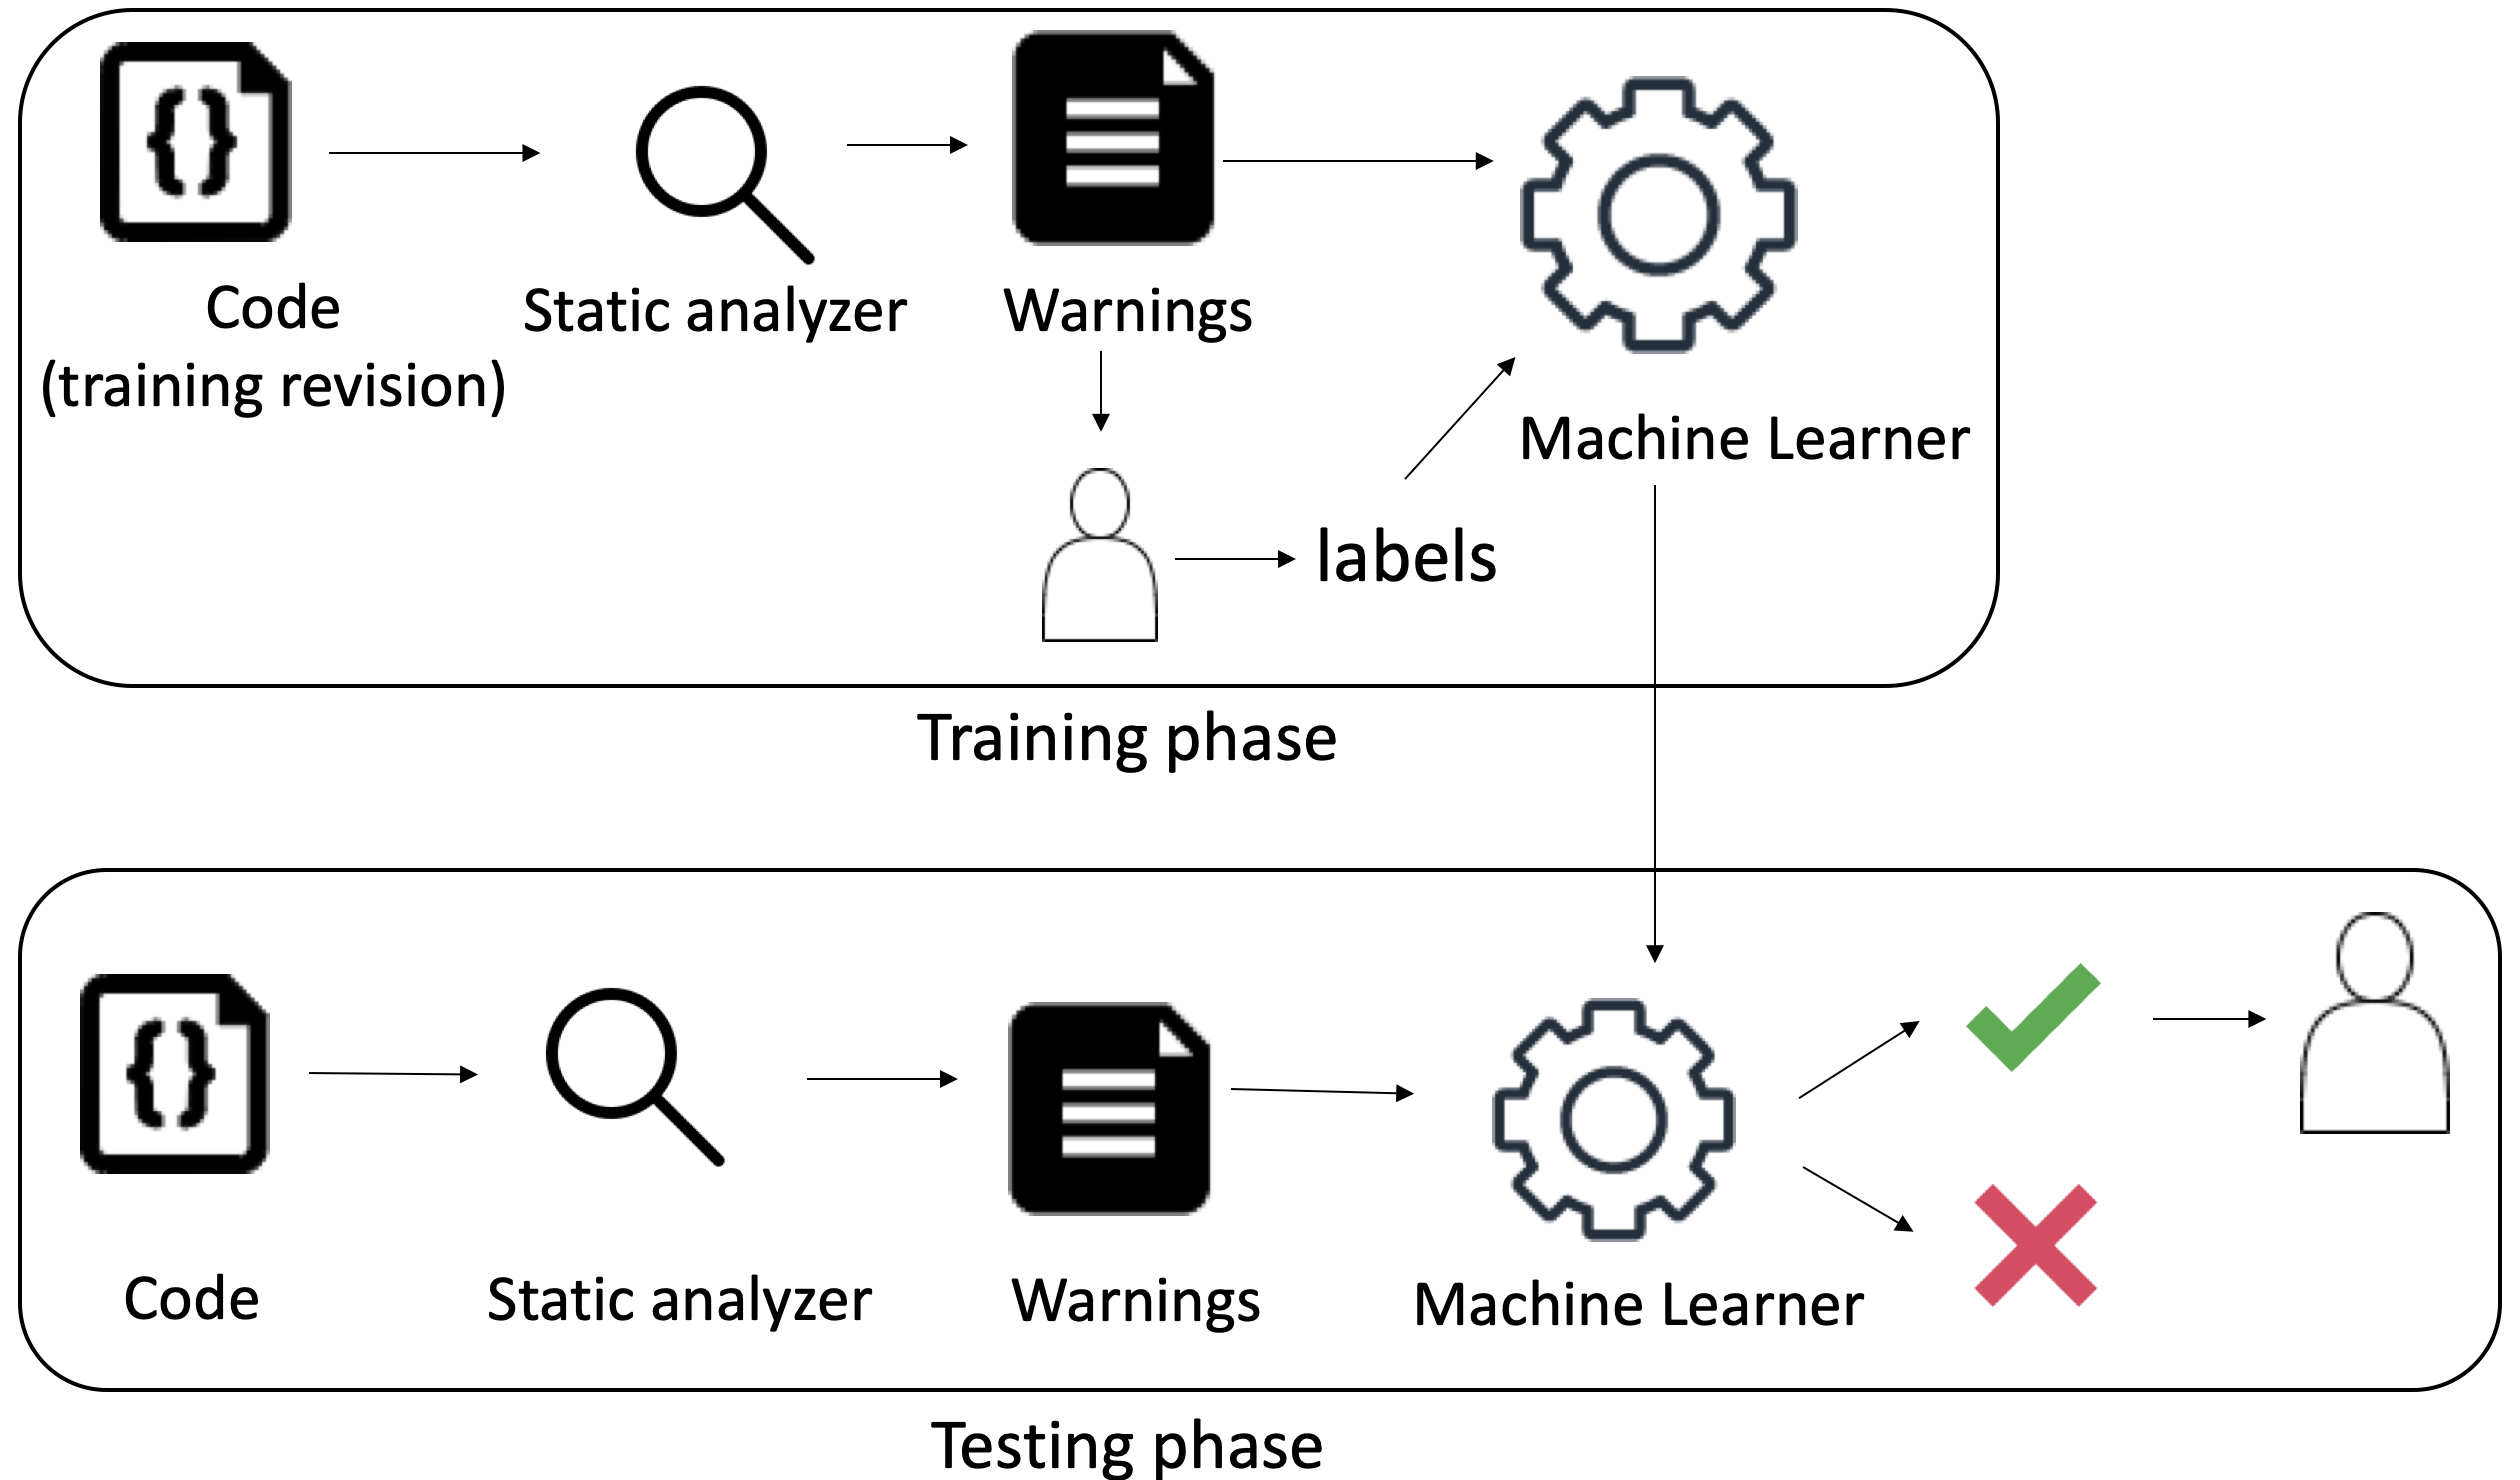
\includegraphics[width=\columnwidth]{hongjin/workflow.png}
  \caption{To detect actionable warnings, a   learner is trained   on warnings from a training revision. Each warning is annotated with a label. When deployed on the latest revision, only warnings classified as actionable warnings by the machine learner are presented to the developers. }
      \label{fig:workflow}
  \centering
  \end{figure}

To assess proposed machine learners, datasets of warnings produced by Findbugs have been created.
As the ground-truth label of each warning is not known, a heuristic was applied to infer them.
This heuristic compares the warnings reported at a particular revision of the project against a revision set in the future.
If a warning is no longer present, but the file is still present, then the heuristic determines that the warning was fixed. 
As such, the warning is actionable.
Otherwise, if the warning is still present, then the warning is a false alarm.


% \begin{table}[t]
% \footnotesize
%   \centering
%   \caption{The features studied in prior work~\cite{wang2018there,yang2021learning,yang2021understanding}. The ``Golden Features'' are in bold.}
%   \label{tab:golden_features}
  
%     \begin{tabular}{l|l}
%       \toprule
%  \textbf{Feature type}     & \textbf{Feature} \\
%  \midrule
%  & size context for warning type, method  \\ 
%  & size context in file, package \\ 
 
%  & \textbf{warning context in method, file}, package   \\
%  & \textbf{warning context for warning type}  \\
%  & fix, non-fix change removal rate \\
%  Warning  & \textbf{defect likelihood for warning pattern} \\
%  combination & variance of likelihood \\
%  & defect likelihood for warning type \\ 
%  & \textbf{discretization of defect likelihood} \\
%  & \textbf{average lifetime for warning type}\\
%  \midrule
%  & method, file, package size\\
%  & comment length \\
%  & \textbf{comment-code ratio} \\
%  & \textbf{method depth}  \\
%   & \textbf{file depth} \\
%  Code  & method callers, callees \\ 
%  characteristics & \textbf{\# methods in file}, package \\
%  & classes in file \\ 
%  & \textbf{\# classes in package} \\
%  & indentation \\ 
%  & complexity \\
%  \midrule
%  & \textbf{warning pattern} \\
%  & \textbf{warning type}  \\
%  Warning  & \textbf{warning priority}  \\
%  characteristics & warning rank, warnings in method, file \\
%  & \textbf{package} \\
%  \hline
%  & latest file, package modification \\ 
%  & file, package staleness \\
%  File & \textbf{file age, creation}  \\
%  history & deletion revision \\
%  & \textbf{developers} \\
%  \hline
%  & call name, class, \textbf{parameter signature} \\
%  & \textbf{method visibility} \\
%  & return type \\ 
%  & new type, new concrete type \\ 
%  & operator \\ 
%  Code  & field access class, field \\ 
%  analysis & catch \\ 
%  & field name, type, visibility, is static/final \\ 
%  & return type \\ 
%  & is static/ final/ abstract/ protected \\ 
%  & class visibility,is interface \\
%  \hline
%  & added, changed, deleted, growth, total,  \\
%  & percentage of LOC in file (past 3 months) \\
%   & LOC \textbf{added} , changed, deleted, growth \\
%  Code  & total, percentage in file (last 25 revisions)\\
%  history &  \textbf{added}, changed, deleted, growth, total,  \\ 
%  & percentage of LOC in package  (past 3 months) \\
%  & added, changed, deleted, growth, total,  \\
%  & percentage of LOC in package (last 25 revisions) \\
% \hline
% Warning  & \textbf{warning lifetime by revision}, by time \\
% history & warning modifications, open revision \\
% \midrule
% File  & file type, name \\
% Characteristics & package name \\
% \bottomrule 
% \end{tabular}


% \end{table}

 Wang et al.~\cite{wang2018there} ran a systematic literature review to collect  and analyze 100+ features proposed in the literature, categorizing them into 8 categories.
To remove ineffective features, they performed a greedy backward selection algorithm.
From the features, they identified a set of features that     offered effective performance.
% Table \ref{tab:golden_features} lists these features.

\subsection{Further Result: Yang et al., 2021}

Yang et al.~\cite{yang2021learning} further analyzed the   features using the data collected by Wang et al.~\cite{wang2018there}. 
They found that all machine learning techniques were effective and performed similarly to one another. 
Their analysis revealed that the intrinsic dimensionality of the problem was low; 
the features used in the experiments were more verbose than the actual attributes required for classifying actionable warnings.
This motivates the use of simpler machine learners over more complex learners.
From their analysis, SVMs were recommended for use in this problem, as they were both effective and can be trained at a low cost.
In contrast, deep learners were effective but more costly to train.

For each project in their experiments, 
one revision (training revision) was selected for extracting warnings for training the learner, 
and another revision (testing revision) set chronologically in the future of the training revision is selected for extracting warnings for evaluating the learner. 
This simulates a realistic usage scenario of the tool, where the learner is trained using past data before developers apply it to  another revision of the source code.



\subsection{Issues in Prior Results: Kang et al., 2022}
Subsequently, Kang et al.~\cite{kang2022detecting} replicated  the Yang et al.~\cite{yang2021learning} study
to find subtle methodological issues in the     Wang et al. data~\cite{wang2018there} which   led to overoptimistic results.

Firstly, Kang et al. found data leakage where the information regarding the warning in the future, used to determine the ground-truth labels,  leaked into several features.
Five features (warning context in method, file, for warning type, defect likelihood, discretization of defect likelihood) measure the ratio of actionable warnings within a subset of warnings (e.g. warnings in a method, file, of a warning type). 
To determine if a warning is actionable, the ground-truth label was used to compute these features, leading to data leakage.
Kang et al.   reimplemented the features such that they are computed using only historical information, without reference to the ground truth determined from the future state of the projects.
As only the features were reimplemented, the total number of training and testing instances remained unchanged.

Secondly, they found many warnings appearing in both the training and testing dataset. 
As some warnings remain in the project at the time of both the training and testing dataset, the model has access to the ground-truth label for the warning at training time.
Kang et al. addressed this issue by removing warnings that were already present during the training revision from the testing dataset, ensuring that the learner does not see the same warning in both datasets.
After removing these warnings, the number of warnings in the testing revision decreased from
15,695 to 2,615.
% 15,363 to 


\begin{table}[t]
    \centering
    \caption{Evaluation metrics based on TP (true positives); TN (true negatives);
    TP (true positives) and FP (false positives)}
    \label{tab:metrics}
      \rowcolors{2}{white}{gray!15}
    \begin{tabular}{rp{5cm}}
        \toprule
        \textbf{Evaluation Metric} & \textbf{Description}  \\
        \midrule
        Precision & $\frac{\text { TP } }{\text {TP}+\text {FP}}$ \\ 
    
        AUC  & area under the receiver operating
characteristics curve (the true positive
rate against the false positive rate) \\ 
   
        False alarm rate & $\frac{\text { FP } }{\text {FP}+\text {TN}}$\\
      
        Recall &  $\frac{\text { TP } }{\text {TP}+\text {FN}}$ \\
        \bottomrule
    \end{tabular}
\end{table}


\begin{table}[!t]
  \centering
  \caption{The Kang et al. predictors did not perform well on the repaired data. In this table,{\em lower} false alarms are better while {\em higher} precisions, AUC, and recall are {\em better}. }
  \label{tab:initial_svm}
  \rowcolors{2}{white}{gray!15}
  \begin{tabular}{rrrrr}
 
 \toprule
                 
 \textbf{Dataset}           &  \textbf{Precision} & \textbf{AUC} & \textbf{False alarm rate} & \textbf{Recall}          \\
  \midrule 
  cassandra & 0.67 & 0.33 & 0.25 & 0.67 \\
   commons & 0.67 & 0.52 & 0.57 & 0.62 \\
   
  lucene-solr & 0.56 & 0.70  & 0.36 &  0.71\\
  
  median & 0.52 & 0.41 & 0.19 & 0.32 \\
  jmeter & 0.50 & 0.36 & 0.14 & 0.17 \\
  
  tomcat & 0.52 & 0.41 & 0.19 & 0.32 \\
  
  derby & 0.20 & 0.64 & 0.12 & 0.08 \\
 
  ant & 0.00 & 0.00 & 0.00 & 0.00 \\
  \bottomrule
  \end{tabular}
  
\end{table}



Next, Kang et al. analyzed the warning oracle, based on the heuristic comparing warnings at one revision to another revision in the future, used to automatically produce labels for the warnings in the dataset. 
After manual labelling of the actionable warnings, Kang et al. found that only  47\% of warnings automatically labelled actionable were considered by the human annotators to be actionable.
This indicates that the heuristic employed as the warning oracle is not sufficiently reliable for automatically labelling the dataset. 

Kang et al. manually labelled 1,357 warnings. After filtering out duplicates and  uncertain labels, a dataset of 768 warnings remained.
On this dataset, Kang et al. again applied  off-the-shelf SVM models, assessing them with the evaluation metrics listed in Table \ref{tab:metrics}. 




For their reasoning, 
Kang et al. used  the learners recommended by prior work;
i.e. radial bias  SVMs.
The results of the SVM are shown in Table \ref{tab:initial_svm}.
Those results are hardly impressive:
\bi
\item Median precisions barely more than 50\%;
\item Very low median AUCs of 41\%;
\item Extremely low median recalls of 32\%.
\ei
That is to say, while Kang et al. were certainly correct
in their criticisms of the data used in prior work, based on their paper,
it is still an open issue about how to   generate good predictors for static code false alarms. 




% In this paper, we build upon the features identified in the prior studies~\cite{hanam2014finding,heckman2008establishing,liang2010automatic,ruthruff2008predicting,wang2018there,yang2021learning,yang2021understanding}; but instead of only using off-the-shelf machine learners, we tap on the power of more advanced and specialized learners, data engineering methods and hyperparameter optimization steps.


%Another aspect of the analysis addressed by Kang et al.~\cite{kang2022detecting} was the dataset. In particular, they analyzed the heuristic used to infer labels. They found that the labels were inaccurate and were not consistent with manually labelled data by human annotators. Moreover, their experiments suggested that the effectiveness of the machine learners vary with different strategies for inferring labels. This points to the need for human involvement in curating warnings for a benchmark dataset and highlights the importance of data quality. In turn, it highlights the need for methods that can effectively learn from small quantities of human annotated data given the high cost of labelling.

 
 



 
\section{Rethinking the Problem}\label{problem}

This section suggests that detecting actionable static code warnings is a ``bumpy'' problem
(defined below) and that such problems can not be understood by learners that use simplistic
boundaries between classes.  

The core task of any classification problem is the creation of a hyperspace
boundary that let us isolate what is most desired or most interesting. Different learners build their boundaries in different ways:
\bi
\item Simple decision tree learners can only build straight-line
boundaries. 
\item Neural networks can produce very complex and convoluted boundaries.
\item And
internal to   
Kang et al.'s support vector machine was a ``radial basis function''
that allowed those algorithms to build circular hyperspace
boundaries.  
\ei 
Boundaries can be changed by adjusting
the
parameters that control the learner. For example, in Kang et al.'s radial basis functions,
the $C$ regularization parameter is used to set the tolerance of the model to (some) classifications. By adjusting $C$, an analyst can change
the generalization error; i.e. the error when the model is applied to as-yet-unseen test data.

Figure~\ref{cg} show how changes to $C$ can alter the decision
boundary between some red examples and blue examples. Note that each
setting to $C$ changes the accuracy of the predictor; i.e.
for good predictions, it is important to fit the shape of the decision boundary to the shape of the data. 

(Technical aside: while this example was based on SVM technology, the same line of argument applies to  any other classifier; i.e. changing
the control parameters of the learner also changes the hyperspace boundary 
found by that learner and, hence, the predictive prowess of that learner.)

We have tried applying    hyperparameter optimization to   $C$ in a failed attempt to improve that performance (see the C1 results of Table \ref{tab:results}). 
From that failed experiment, we conclude that   however  $C$ work
for radial bias functions, they do not work well enough to fix
the unimpressive predictive performances -- see Table~\ref{tab:initial_svm}.


 

Why do radial bias SVMs fail in this domain?  Our  conjecture is that the hyperspace boundary dividing the static code examples (into false positives and others)
is so ``bumpy''\footnote{``Bumpy'' data 
  contain complexities such
as many local minima, saddle points, very flat regions,
and/or widely varying curvatures. For example, see  Figure \ref{fig:loss}.}
that the kinds of shape changes seen
in   Figure~\ref{cg} can never adequately model those  examples.

\begin{figure}[!t]
 \noindent {\footnotesize \begin{tabular}{c@{}c@{}c}
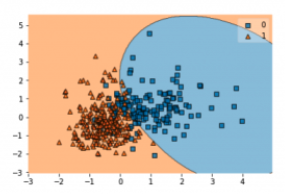
\includegraphics[height=.8in]{rahul/c0_1g0_1.png}&
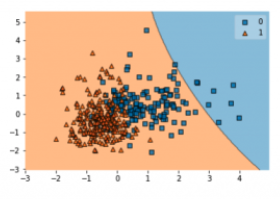
\includegraphics[height=.8in]{rahul/c0_1g0_008.png}&
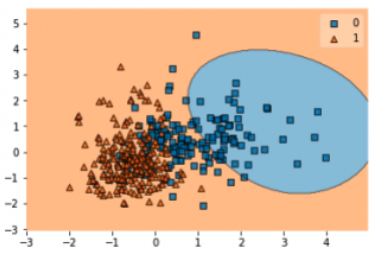
\includegraphics[height=.8in]{rahul/c0_02g_01.png}\\
$C=0.1$&$C=0.1$&$C=0.2$\\ 
$\mathit{acc}=90\%$& $\mathit{acc}=64\%$&  $\mathit{acc}=81\%$ 
\end{tabular}}

\caption{The $C$  parameter of a radial basis function alters
the shape of the hyperspace boundary.  {\em Acc} is accuracy which is the ratio of true positives plus true negatives divided by a SVM making predictions across that boundary. Example from~\cite{kumar20}.}\label{cg}
\end{figure}

To test that conjecture, we first    checked for ``bumpiness" using a technique
from \citet{li2018visualizing}. That technique
visualizes the ``error landspace'' 
(i.e. how fast small changes in the independent variables altered the error
estimation).
% The technique is in two parts:
% \bi
% \item A way to reduce N-dimensional data to two-D plot, plus a third
% dimension to represent the loss function (e.g. see Figure \ref{fig:loss}a); 
% \item
% A  statistic that Li calls ``$\beta-$smoothness''
% that measures
% the simplicity of that landscape\footnote{According to \citet{li2018visualizing}, given some error function $f$ and samples at point $x$,
% $\beta-$smoothness is defined as the maximum value of $\beta$ for which $\lVert \nabla f(x_1) - \nabla f(x_2) \rVert \leq \beta \lVert x_1 - x_2 \rVert$ under some norm (we use the $l_2$ norm), and is a measure of the smoothness of the loss surface (i.e., higher the $\beta-$smoothness, smoother the error surface).}. 
% \ei
For our TOMCAT data, Li et al.'s methods resulted in Figure \ref{fig:loss}.
There, we see a ``bumpy'' landscape
with several multiple local minima. 
% The presence   multiple minima means that, in different local  regions of the data,
% we will need different adjustments to the hyperspace boundary.  

Having confirmed that our data is ``bumpy'', our second step was to
we look  for ways to reduce that bumpiness. Initially, we attempted to use
  neural nets since that kind of learner is meant
to be able to handle complex hyperspace boundaries~\cite{WittenFH11}.
As discussed in \S\ref{sec:results}, that attempt failed even after trying
several different architectures such 
as
feedforward networks, CNN,  and CodeBERT~\cite{rumelhart1986learning,habib2018many,vaswani2017attention}
(with and without tuning learner control parameters).

Since standard neural net technology failed, we tried several   manipulation techniques for the training process, described in the next section.  

\begin{figure}[!t]
   \begin{center}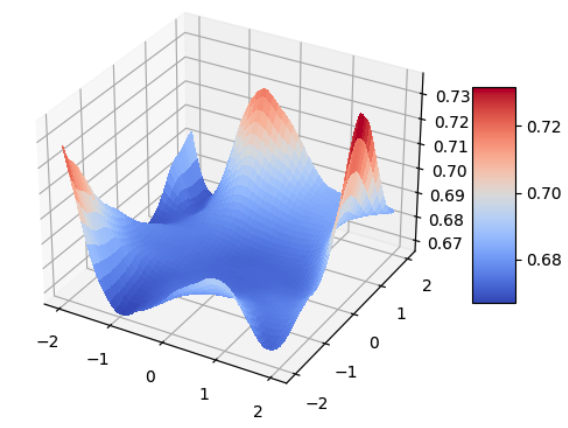
\includegraphics[width=.3\textwidth]{rahul/pre1.png} \end{center}
 
    \caption{Error landscape in the TOMCAT data    before    applying the methods of this paper. In the plot, the larger the vertical axes, the greater the loss value.
    Later in this paper,
    we will show this plot again, after it has been smoothed via the   methods of  \S\ref{rx}
    (see Figure~\ref{fig:gain} and Table~\ref{tab:fuzzy}).}
    \label{fig:loss}
\vspace{-10pt}
\end{figure}

\section{  Treatments}\label{rx}

 This section discusses a framework that holds
 operators for   treating the data in order to adjust  the decision boundary (in different ways for different parts of the data). For the purposes of illustration and experimentation,
 we offer operational examples for each part of the framework:
 \bi
 \item  SMOTE for instance engineering;
 \item  SMOOTH for label engineering;
 \item   GHOST for boundary engineering;
 \item   DODGE for parameter engineering.
 \ei
 Before presenting those parts we note here that the framework is more than just those four treatments. 
 As SE research matures, we foresee that our framework will become a workbench   within which researchers replace some/all of these treatments with more advanced options.
 
 That said, we have some evidence that  SMOTE, SMOOTH, GHOST, DODGE are useful:
 \bi
  \item
The ablation study of \S\ref{rigg}  shows that removing any one of these treatments leads to worse performance.
 \item
All these treatments are  very fast: sub-linear time for SMOTE and SMOOTH, linear time for GHOST, and DODGE is known to be orders of magnitude faster than other hyperparameter optimizers~\cite{agrawal2019dodge}.
 \ei


 

\subsection{Instance Engineering (via SMOTEing)}
To remove the ``bumpiness'' in data like Figure~\ref{fig:loss}, we need to 
pull and push the decision boundaries between different classes into a smoother shape.
But also, unlike simplistic $C$ tuning available in radial  SVMs, we want that process to perform differently
in different parts of the data.

One way to adjust the decision boundary in different parts of the data is 
to add (or delete)  artificial examples around each example $X$. This builds a little ``hill'' (or valley) in the local region.
As a result, in that local region,
 it becomes more (or less)
certain that all predictions which reach the same conclusion as $X$. In effect, adding/deleting
examples pushes the decision boundary away (or, in the case of deletions, pulls it closer).
SMOTE \cite{chawla2002smote} is one instance engineering technique that:
\bi
\item Finds  five nearest neighbors
to   $X$ with the same label;
\item  Selects one at random;
\item Creates a new example $R$, with the same label as $X$ at some random point
between $X$ and $R$.
\ei

\subsection{Label Engineering (via SMOOTHing)}

SMOTE has seen much success in recent SE papers as a way to improve predication efficacy~\cite{agrawal2018better}. 
But this technique makes a {\em linearity} assumption that all the data around $X$ is correctly labelled
(in our case, as examples of actionable or unactionable static code warnings).
This may not be true.
 \citet{cordeiro2020survey} and recent SE researchers~\cite{frugal, debtfree, 9064604, jitterbug} note that  noisy labels can occur when human annotators are present~\cite{mcnicol2005primer} or those humans  have divergent opinions about the labels~\cite{barkan2021reduce, ma2019blind}. Although our labels were re-checked by the authors of \citet{kang2022detecting}, our ablation study (below) reports that it is best to apply some
 mitigation method for 
 poorly labelled examples. For example, in this work we applied the following SMOOTHing   operator where data is assigned labels using multiple near neighbors. This has the effect of removing outliers in the data. 
 Our SMOOTH operator works as follows:
 \bi
 \item
 Given $n$ training samples (and therefore, $n$ labels), we keep $\sqrt{n}$ at random and discard the rest.
 \item
 Next, we use  a KD-tree to recursively sub-divide the remaining data into leaf clusters of   $\sqrt[4]{n}$ nearest neighbors. Within each leaf, all examples are assigned a label that is the  mode of the labels in that leaf.
 \ei
 One interesting and beneficial side-effect of SMOOTHing is that we   make conclusions on our test data using just 10\% of the training data. 
  By reducing  the labelling required to make conclusions, SMOOTHing
 offers a way to help future studies avoid the problems reported by Kang et al.~\cite{kang2022detecting}:
 \bi
 \item   One of the major finding of the Kang et al. study was that earlier work~\cite{yang2021learning}  had mislabelled much of its data. From that study, we assert that it is important for analysts to spend more time checking their labels.
 We note that there many other ways to reduce the labels required for supervised learning. 
%  In future work, we will explore {\em semi-supervised learning}~\cite{Tu21} methods, seeking ways to make conclusions using as few labels as possible.
 \item SMOOTHing reduces the effort required for that checking
 process (by a factor of ten).
 \ei
 As an aside, we note that SMOOTHing
 belongs to a class of algorithms
 called {\em semi-supervised learning}~\cite{frugal, debtfree}  that try to   make conclusions using as few labels as possible.
The literature on semi-supervised learning is voluminous \cite{berthelot2019mixmatch, fairssl, kingma2014semi,  zhai2019s4l, zhu2005semi} and so, in the theory, there could be many other better ways to perform label engineering.
This would be a productive area for future research.    But for now, the ablation
  study (reported below) shows that   SMOOTHing is useful
  (since removing it degrades predictive performance).
  

\subsection{Boundary Engineering (via GHOSTing)}

As defined above, instance and label engineering do not reflect on the quality of data in the local region.

To counter that, this study employs a boundary method called ``GHOSTing'', recently developed and applied to software defect prediction  by    \citet{yedida2021value}.
 Boundary engineering is different to label and instance engineering since it adjusts the frequency of different classes
 in the local region (while the above typically end up repeating the same label for a particular locality). Hence, in that region,
 it changes the decision boundary. 
 
 
GHOSTing addresses class imbalance issues in the data.   When an example with one label
is surrounded by too many examples of another label, then the signal associated with
example can be drowned out by its neighbors
To fix this,
for a two-class dataset $D$ with class $c_0$ being the minority, GHOSTing oversamples the class by adding concentric boxes of points around each minority sample. The number of concentric boxes is directly related to the class imbalance: higher the imbalance, more the number of boxes. Specifically, if $n$ is the fraction of samples in the minority class, then $\lfloor \log_2 (1/n) \rfloor$ boxes are added.
While the trivial effect of this is to oversample the class (indeed, as pointed out by \citet{yedida2021value}, this \textit{reverses} the class imbalance), we note that the algorithm effectively builds a wall of points around minority samples.
This pushes the decision boundary away from the training samples, which is preferred since a test sample that is close to a training sample has a lesser chance of   being
misclassified due to the decision boundary being in between
them.

Our pre-experimental intuition was that  boundary engineering would replace the need to use instance engineering. However, as shown by our ablation study, for recognizing actionable static code warnings, we needed both tools. On reflection, we realized   both may be  necessary since while (a)~boundary engineering can help make local adjustments to the decision boundary, it can (b)~only work in regions where samples \textit{exist}; instance engineering can help fill in gaps in sparser regions of the dataset.


\begin{table}[!t]
    \centering
    \caption{List of hyper-parameters tuned in our study.
    CodeBERT is not shown
  in that table since, as mentioned in the text, this analysis lacked
  the resources required to tune such a large model.}
    \label{tab:hyperparams}
    
   
    \begin{tabular}{llp{2.2cm}}
        \toprule
        \textbf{Learner} & \textbf{Hyper-parameter} & \textbf{Range}  \\
       
 \rowcolor{gray!15}         Feedforward network & \#layers & $[2, 6]$ \\
  \rowcolor{gray!15}        & \#units per layer & $[3, 20]$ \\
        
       Logistic regression & Penalty & $\{l_1, l_2\}$ \\
        & C & $\{0.1,1,10,100\}$ \\
        
  \rowcolor{gray!15}     Random forest & Criterion & $\{$ gini, entropy $\}$ \\
   \rowcolor{gray!15}       & n\_estimators & $[10, 100]$ \\
        
       Decision Tree & Criterion & $\{$ gini, entropy $\}$ \\
        & Splitter & $\{$ best, random $\}$ \\
         
  \rowcolor{gray!15}     SVM & C & $\{0.1,1,10,100\}$ \\
   \rowcolor{gray!15}       & Kernel & $\{$sigmoid, rbf, polynomial $\}$ \\
   
   CNN & \#convolutional blocks & [1, 4] \\
   & \#convolutional filters & \{4, 8, 16, 32, 64\} \\
   & Dropout probability & (0.05, 0.5) \\
   & Kernel size & \{16, 32, 64\} \\
        \bottomrule
    \end{tabular}
\end{table}
        

\subsection{Parameter Engineering (via DODGEing)}

We noted above that different learners
generate different hyperspace
boundaries (e.g. decision learners generate
straight-line borders while SVMs with radial bias functions generate circular borders). Further, once a learner
is selected, then as seen in Figure \ref{fig:loss}, 
it is possible to further adjust
a border by altering the   control parameters of
 that learner (e.g. see Figure~\ref{cg}).  We call this adjustment
 {\em parameter engineering}.
 
 Parameter engineering is like a scientist probing some phenomenon. After the data is divided into training and some
 separate test cases, parameter engineering algorithms conduct experiments on the training data looking for parameter settings
 that improve the performance of a model learned and assessed
 on the training data. Once some conclusions are
 reached about what parameters are best, then these are applied
 to the test data. Importantly, the parameter engineering  should only use the training    data for its investigations (since otherwise, that
 would be a threat to the external validity of the conclusions).
 
 
 Parameter engineering executes within the
 space of control parameters of selected learners. 
   These learners have the internal parameter space shown 
  in Table~\ref{tab:hyperparams}. 
We selected this range of learners using the following rationale:
 \bi
 \item
   In order to   compare our new results to   prior work by Kang et al. ~\cite{kang2022detecting}, we use the 
   Kang et al. {\em   SVMs}
  with the radial basis kernel and balanced class weights.
\begin{table}[!b]
    \centering
    \caption{Neural net architectures used
    in this study.}
    \label{tab:nnhere}
    
      \small
    \begin{tabular}{p{8.5cm}}
        \toprule
    \rowcolor{gray!15}
     {\em Feedforward networks}
     These are   artificial neural networks, comprising an acyclic graph of nodes that process input and produce an output. These dates back to the 1980s, and the parameters of these models are learned via backpropagation \cite{rumelhart1986learning}. 
       These networks have $\mathcal{O}(10^3)-\mathcal{O}(10^4)$ parameters. 
     For these networks, we used the    ReLU  (rectified linear activation)    function ($f(x) = \max (0, x)$).
     This is a  piecewise linear function that will output the input directly if it is positive, otherwise, it will output zero.  
        ~\\
        A {\em convolutional neural net} (CNN) is a structured neural net where the first several layers are sparsely connected in order to process information (usually visual).
        CNN is an example of an  
        {\em deep learner} and  are much larger than
        feedforward networks (these may   span $\mathcal{O}(10^5)-\mathcal{O}(10^7)$ parameters).
        Optimizing an CNN is a very complex task (so many parameters) so
        following   advice from the literature~\cite{ioffe2015batch,srivastava2014dropout}, we used the following architecture. Our CNNs had multiple ``convolutional blocks'' defined as follows:
\begin{enumerate}
    \item ReLU activation
    \item Conv (with ``same'' padding)
    \item Batch norm \cite{ioffe2015batch}
    \item Dropout \cite{srivastava2014dropout} 
\end{enumerate}

We note that this style of building convolutional networks, by building multiple ``convolutional blocks'' is very popular in the CNN literature \cite{krizhevsky2012imagenet,lecun1989backpropagation}. 
Our specific design of the convolutional blocks was based on a highly voted answer on Stack Overflow \footnote{\url{https://stackoverflow.com/a/40295999/2713263}}.

Note that with that architecture there is
still room to adjust the ordering of the blocks-- which is what we adjust when we tune our CNNs.\\   \rowcolor{gray!15} 
CodeBERT~\cite{feng2020codebert} is a {\em transformer-based}  model that been   pre-trained model using millions of examples
 from contemporary programming languages such as Python, Java, JavaScript, PHP, Ruby, and Go. 
Such transformer models
are those based on the ``self-attention'' mechanism proposed by \citet{vaswani2017attention}. CodeBERT
        is even large than CNN and can contain $\mathcal{O}(10^8)-\mathcal{O}(10^9)$ parameters.
One advantage of such large models is that can 
 learn intricacies that are missed by smaller models.   \\\bottomrule
    \end{tabular}
\end{table}    
 \item
   In order to   compare our   work to    Kang et al. ~\cite{yang2021learning}, we used 
  a range of  {\em traditional learners}
  (logistic regression, random forests, and single
 decision tree learners); 
 \item
Also, we explored the various  {\em    neural net algorithms}
shown in  Table~\ref{tab:nnhere}
since these algorithms have a reputation
 of being able to handle complex decision boundaries~\cite{WittenFH11}. 
 In this textbook on {\em Empirical
     Methods for AI}, Cohen~\cite{cohen1995empirical} advises that supposedly more complex solutions should be compared to  a range of alternatives, including very
     simple methods. Accordingly, for neural nets,
     we used (a)~feedforward networks from the 1980s;
     (b)~the CNN deep learner used in much of contemporary SE
     analytics; and (c)~the state-of-the-art   CodeBERT model.
 \ei     
% \noindent
% {\bf RQ6}  is an interesting questions since before we recommend complex algorithms,
% it is prudent to ask if that complexity is required. We say this since the cost to commission different kinds of machine learners can vary by orders of magnitude.
% For example, DODGE requires 3 seconds and 3 hours (respectively) to tune feedforward networks and CNN, respectively
% (and CODEBERT is so complex that we cannot tune it all). 
% which makes optimization difficult. To fix this, we look at prior work that successfully applied deep learning in software engineering. One such study was the GHOST study by \citet{yedida2021value}, which used a combination of hyper-parameter optimization and a novel ``fuzzy sampling'' technique. That study described the necessity of fuzzy sampling as pushing the decision boundary away from training samples so that test samples are not misclassified if they are close to a training sample, yet separated by the decision boundary. While this was convincing, we were motivated by the spirit of a study by \citet{santurkar2018does}, who showed that Batch Normalization \cite{ioffe2015batch} worked because it smoothens the surface of the loss function. Does fuzzy sampling have a similar effect? We tested this by applying fuzzy sampling as discussed by \citet{yedida2021value} and then redrawing the loss landscape. This led to Figure \ref{fig:loss}b, which is significantly smoother. We observed a similar trend across all our datasets
% its losses   loss function ss functions are   algorithm that summarizes the performance of test test. Loss functions are entire
% field of research on to themstemselves. For examle,
% the cross-entr
% non-convex. Could this non-convexity explain why these
% in the paper
% and  report here that the
% For that  purpose   (local adjustment of the separation policy), we will use {\em instance, label, boundary}
% and {\em parameter} engineering methods described in the next section.% Methods that adjusts   data   to enhance learning needs to show    that they avoid the following threat to validity:
% \bi
% \item
% A learned model must be tested on the kinds of data expected in practice (and not some artificially mutated set). 
% \iten
% Hence, it is vital to assert that
% {\em any data manipulations  are restricted to the training data, and do {\bf not} effect the test  data.}
% \ei
% We assert that in the following, our data manipulations are restricted {\bf only} to   training data.
% \subsection{Why prior work fails }
% To begin, we reflect on why prior approaches did not perform well. The prior study used SVMs, which rely on convex optimization to create a maximum-margin classifier in a kernel space (the prior study used the radial basis function kernel). Noise in the dataset can mean that this optimization problem can be fundamentally difficult. Further, parameters such as $\gamma$ and $C$ of SVMs can only affect the \textit{global} shape of the decision boundary, while we desire changes to the \textit{local} (per-sample) shape of the decision boundary (without overfitting). To tackle this, we leverage classifiers whose decision boundaries can take on arbitrary shapes, i.e., feedforward networks, which are universal approximators \cite{cybenko1989approximation, hornik1989multilayer}.
% However, feedforward networks, even when tuned, may perform poorly. We notice that feedforward networks work by optimizing a loss function, which is typically non-convex. Could this non-convexity explain why these learners struggle to learn a good decision boundary? To test this, we explore the topology of the loss landscape. Specifically, we use the technique of \citet{li2018visualizing} to visualize the landscape of our loss function. On examining these plots (see Figure \ref{fig:loss}a for an example), we see a rough landscape with several local minima, which makes optimization difficult. To fix this, we look at prior work that successfully applied deep learning in software engineering. One such study was the GHOST study by \citet{yedida2021value}, which used a combination of hyper-parameter optimization and a novel ``fuzzy sampling'' technique. That study described the necessity of fuzzy sampling as pushing the decision boundary away from training samples so that test samples are not misclassified if they are close to a training sample, yet separated by the decision boundary. While this was convincing, we were motivated by the spirit of a study by \citet{santurkar2018does}, who showed that Batch Normalization \cite{ioffe2015batch} worked because it smoothens the surface of the loss function. Does fuzzy sampling have a similar effect? We tested this by applying fuzzy sampling as discussed by \citet{yedida2021value} and then redrawing the loss landscape. This led to Figure \ref{fig:loss}b, which is significantly smoother. We observed a similar trend across all our datasets. 
% So far, our discussion walked through the application of essentially, the GHOST system proposed by \citet{yedida2021value}. We studied the efficacy of this approach (see the A5 treatment in our results, Figure \ref{fig:results}). While this was promising (median AUC = 0.83), we felt that there was room for improvement. To accomplish this, we went to the root of this paper: working with the manually labeled dataset by \citet{kang2022detecting}. What if this dataset was also noisy? This led us to experiment with a novel, but simple, semi-supervised learning approach which does not trust the labels given. Specifically, we used the label engineering methods of \S \ref{sec:labelengineering}. Adding this yielded our final technique, which we call GHOST2 (see treatment A1 in our results).
% It is worth reflecting further over our approach. While GHOST2 can be thought of as GHOST + label engineering, it is worth noting that GHOST itself is a box containing multiple layers of engineering techniques. Specifically, it consists of fuzzy sampling--which is intended to push the decision boundary away, what we call ``boundary engineering'', hyper-parameter optimization, which we simply relabel as ``hyper-parameter engineering'', and SMOTE, which adds in points between two samples of the same class--what we call, ``instance engineering''. Our takeaway from this discussion is:
% \begin{quote}
%     {\em Learning problems should be treated as a set of engineering decisions, which should be individually tended to, rather than using tools off-the-shelf.
%     }
% \end{quote}
% We start by discussing the solution to the problem of global decision boundary engineering (via, for example, the $C$ and $\gamma$ parameters). We will seek out learners that can, informally, create human-like decision boundaries (i.e., boundaries that fit the data well, with locally-adjusted modifications, without overfitting).
% \subsection{Learner Choice}
% \label{sec:learner}
% Modern machine learning offers a plethora of learning algorithms, especially in the supervised setup. We classify these learners  into 
% {\em traditional} and {\em neural} approaches.  Further, we divide neural approaches into {\em feedforward} networks, {\em deep learners}, and {\em transformers} \cite{vaswani2017attention}:
% Before proceeding further, it is worth reflecting on why we choose neural approaches to produce locally-adjusted decision boundaries. To do so, we look at \textit{universal approximation theorems} (UATs), theorems that define conditions under which specific learners can approximate any function (i.e., decision boundary) with any arbitrary precision. The first such theorem was by \citet{cybenko1989approximation}, who showed that superpositions of sigmoidal functions (i.e., such as feedforward networks with the sigmoid activation function) are universal approximators. Later, \citet{dasgupta1992power} showed that a set of activation functions had the same approximation power as the sigmoid activation. At the same time, \citet{leshno1993multilayer} showed that feedforward networks with non-polynomial activation functions were universal approximators, and \citet{hornik1991approximation} showed that feedforward networks with non-constant, unbounded activation functions were universal approximators. Therefore, there is a significant body of theoretical evidence that feedforward networks with the ReLU ($f(x) = \max(0, x)$) activation function, which is unbounded and non-constant, can approximate any decision boundary to any desired precision. This makes the feedforward architecture a strong candidate for the choice of learner.
% Following the advice of  \citet{montufar2014number}, we
% configured our CNNS as a  deep ReLU feedforward network is piecewise linear, and go on to provide the lower bound on the number of linear regions in that boundary. That lower bound depends on $\prod\limits_{i=1}^{L-1} \lfloor \frac{n_i}{n_0} \rfloor$, where $L$ is the number of layers in the network, and $n_i$ is the number of units in layer $i$. Clearly, if $n_i < n_0$ for any layer $i$, this lower bound vanishes, and therefore the network is not obliged to try to produce an effective decision boundary. This influences our set of hyper-parameters used in hyper-parameter engineering (discussed later).
% We note that the different kinds of learners enumerated above have different numbers of tuneable parameters. 
% A modern convolutional network can have 100-1,000 times more parameters than a feedforward network (in our experiments, the convolutional networks had $10^5-10^6$ parameters, while the feedforward networks had $10^3-10^4$ parameters). This is significant since it changes the amount of computation needed, and therefore, the amount of time required to train the models.
% To test the effect of learner choice, the experiments described below use representative learners from each category. Specifically, for traditional learners, we use the classifiers from the original DODGE study \cite{agrawal2019dodge}. For feedforward networks, we use a network designed to have a nontrivial decision boundary as discussed above. For deep learners, we use a CNN (whose architecture we will discuss below). Finally, for Transformer-based methods, we use CodeBERT \cite{feng2020codebert}. For all learners except CodeBERT, we attempt hyper-parameter optimization (for CodeBERT, running just once was slow enough to deter us from attempting the multiple repeats necessary for hyper-parameter optimization).
% We use hyper-parameter optimization, passing in the number of convolutional blocks as a hyper-parameter, to find a suitable architecture. 
% Hitherto, we have left a lot of choices of hyper-parameters to hyper-parameter engineering. We discuss the details of this now.
% \subsection{Parameter Engineering}
There are many algorithms currently available for automatically
tuning these learning control parameters.  
As recommended by a prior study \cite{agrawal2021simpler}, we use Agrawal et al.'s  DODGE algorithm~\cite{agrawal2019dodge}. 
DODGE is based on early work by Deb et al. in 2005 that proposed
a ``$\mathcal{E}$-domination rule''~\cite{Deb05}; i.e. 
\begin{quote}
{\em 
If one setting to an optimizer yield results within $\mathcal{E}$
or another, then declare the region $\pm\;\mathcal{E}$ as ``tabu''
and search elsewhere.}
\end{quote}
A surprising result from  Agrawal et al.'s research was that
$\mathcal{E}$ can be very large. 
Agrawal et al. noted that if learners were run 10 times, each time using 90\% of the training data (selected at random), then they often exhibited a  standard deviation of 0.05 (or more) in their performance scores.  Assuming that performance differences less than ${\pm}2\mu$, are
statistically insignificantly different, then Agrawal reasoned that   
$\mathcal{E}$ could be as large as $4*.05=0.2$.
This is an important point.
Suppose we are trying to optimize
for two goals (e.g. recall and false alarm). Since those
measures have
the range zero to one, then
$\mathcal{E}=0.2$ divides the output space of those two goals divides into just a $5{\times}5=25$ regions. Hence, in theory,  DODGE could find good
optimizations after just a few dozen random samples to the space of possible configurations.

When this theoretical prediction was checked
experimentally of SE data, Agrawal~\cite{agrawal2021simpler}  found that DODGE with 
$\mathcal{E}=0.2$ defeated traditional single-point cross-over genetic algorithms as well as state-of-the-art optimizers
(e.g. Bergstra and Bengio's HYPEROPT algorithm~\cite{Bergstra12}\footnote{At the time of this writing (April 2022), the paper proposing HYPEROPT has 7,557 citations in
Google Scholar.}).  Accordingly, this study used DODGE for its parameter engineering.




Our pre-experimental intuition was that DODGEing would
be fast enough to tune even the largest neural net model. This turned out not to be the case. The resources required
to adjust the CodeBERT model are so large that, for this
study, we had to use the ``off-the-shelf'' CodeBERT.



% \subsection{Instance engineering}

% Boundary engineering is a class of techniques that intentionally modify the dataset with the intention of affecting the decision boundary in some way. In our case, that effect was to push the decision boundary away from the training set.

% Subtly different from boundary engineering, we define \textit{instance engineering} as techniques that modify the instances (i.e., add/remove instances). For example, preprocessing algorithms such as normalizing data fall under instance engineering, since the inherent goal is not to modify the decision boundary, but to make optimization easier. SMOTE \cite{chawla2002smote} is another such technique that adds points in between two points of the same class at random. Inherently, SMOTE is meant for oversampling, and has not been studied (to the best of our knowledge) for manipulating decision boundaries. Indeed, SMOTE makes the (sometimes wrong) assumption of piecewise linear decision boundaries; if it generates an artificial sample that the decision boundary must now curve around, it impedes any boundary engineering done. For this reason, we augment standard instance engineering (with SMOTE) with the boundary engineering technique described above.



% \subsection{Boundary Engineering}

% Drawing inspiration by work of ~\citet{montufar2014number}, we say that ``boundary engineering'' is the approximation, then manipulation
% of the decision boundary.

% We characterize the decision boundary as one of the aspects of learning algorithms that can be engineered. Certainly, kernel methods are one such technique for doing so; however, we take an alternative approach, borrowing the fuzzy sampling technique from \citet{yedida2021value}. Briefly, for a two-class dataset $D$ with class $c_0$ being the minority, we can oversamples the class by adding concentric boxes of points around each minority sample. The number of concentric boxes is directly related to the class imbalance: higher the imbalance, more the number of boxes. While the trivial effect of this is to oversample the class (indeed, as pointed out by \citet{yedida2021value}, this \textit{reverses} the class imbalance), we note that the algorithm effectively builds a wall of points around minority samples.
% This pushes the decision boundary away from the training samples, which is preferred since a test sample that is close to a training sample has a lesser chance of being misclassified due to the decision boundary being in between them.


% Boundary engineering makes local changes to the decision boundary, but it alone does not suffice. Among other issues, it creates a class imbalance that must be fixed. Further, if there is a region with no data samples, then boundary engineering does not work in that region. Therefore, we must use an \textit{instance engineering} technique that solves these issues. The next section discusses this.

% \begin{figure}
%     \centering
%     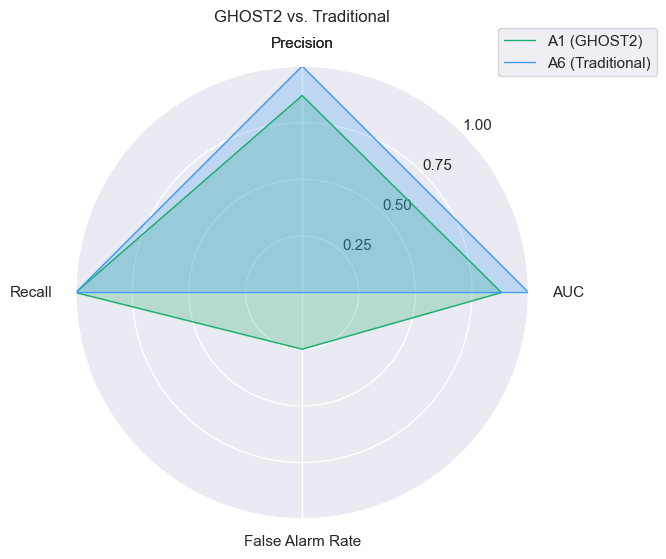
\includegraphics[width=\linewidth]{rahul/comparison.png}
%     \caption{A comparison between A1 (GHOST2), which uses feedforward networks with 9.4\% labels, vs. A6, which uses traditional learners with all the data. Values shown are the medians across 8 datasets. IoU = 0.67}
%     \label{fig:radar}
% \end{figure}





% So far, we have discussed techniques that add in additional data samples to the training set. However, if the original training set is small, as is the case with our datasets, this can lead to the learner over-prioritizing outliers, which can lead to poor performance. We fix this with \textit{label engineering}.


% \subsection{Label Engineering}
% \label{sec:labelengineering}

% Learning algorithms often make assumptions about the data, such as all of it coming from the same distribution. An inherent assumption is also that the labels are correct; but as pointed out by \citet{cordeiro2020survey}, this is often not true. For example, noisy labels can occur when human annotators are present \cite{mcnicol2005primer} and have divergent opinions, as seen in medical images \cite{barkan2021reduce, ma2019blind}. Although our labels were re-checked by the authors of \citet{kang2022detecting}, we assume that some labels are noisy. To rectify the situation, we attempt a simple kind of semi-supervised learning, following Occam's razor. First, given $n$ training samples (and therefore, $n$ labels), we keep $\sqrt{n}$ at random and discard the rest. Next, for each ``unknown'' label, we look at the $\sqrt{\sqrt{n}} = \sqrt[4]{n}$ nearest labels. We take the mode of these labels and assign it as the label for that point. This has the effect of removing outliers in the data. While primitive, our ablation study (of Figure \ref{fig:results})
% confirms that this indeed helps our learning process and improves results. Therefore, we caution researchers to not trust the labels they are given. The details of the number of labels used is given in Table \ref{tab:data}. From the table, we use 58 / (58+554) = 9.5\% labels (which, as we describe later, is $\sqrt{n}$ labels per dataset).






\section{Experimental Methods}
\label{sec:methods}
 



 \subsection{Data}
This paper tested the efficacy of instance, label,
boundary and parameter engineering using the revised
and repaired data from 
  Kang et al. paper~\cite{kang2022detecting}.
  
  Recall that
Kang et al. manually labelled warnings from the same projects studied by Yang et al.~\cite{yang2021learning} to assess the level of agreement between human annotators and the heuristic.
The manual labelling was performed by two human annotators. 
One annotator is an undergraduate student, while the other is a graduate student with two years of industrial experience.
When the annotators disagreed on the label of a warning, they discussed the disagreement to reach a consensus. 
While they achieved a high level of agreement, achieving a Cohen's Kappa of above 0.8, 
manual labelling is costly, requiring human analysis of both the source code and the commit history of the code.
That said, considering the subsequent evolution of the source code allows the annotators to analyze each warning with a greater amount of context.
% That said, this 
These labels are essential
% label is essential 
since it removed closed warnings which are not actionable (e.g., the warnings may have been removed for reasons unrelated to the Findbugs warning). 

Two other filters employed by Kang et al. where:
\bi
\item
Unconfirmed actionable warnings were removed;
\item
False alarms were randomly sampled to ensure a balance of labels (40\% of the data were actionable) consistent with the rest of the experiments.
\ei
One of the complaints of the Kang et al. paper~\cite{kang2022detecting}  against
earlier work~\cite{yang2021learning} was that, for data that comes with some time stamp, it is inappropriate to use future data to predict past labels. To avoid that problem,
in this study, we sorted the Kang et al. data by   time stamps,
then used 80\% of the past data to predict the remaining 20\% future labels.



The Kang et al. data comes from eight projects and we analyzed
each project's data separately. The 80:20 train:test splits
 resulted in the train:test sets shown in Table~\ref{tab:data}
 (exception: for MAVEN, we split 50:50, since there are only 4 samples in total). 
 

Prior studies on static analysis warnings have worked with datasets with a wide range of actionable warnings. For example, Heckman and Williams~\cite{heckman2008establishing} experimented on 2 datasets, one of which had a percentage of actionable warnings of 89\%. 
Imtiaz et al.~\cite{imtiaz2019developers} experimented on several datasets, one of which had a percentage of 49.5\% of actionable warnings. 
Therefore, the percentage of actionable warnings in our experiments is consistent with some prior studies. 

 
Pre-experimentally, we were concerned that learning from the smaller data sets of Table~\ref{tab:data} would complicate
our ability to make any conclusions from this data.
That is, we needed to know:

\begin{formal}\noindent
\rqn{5} \textit{Are larger training sets necessary (for the task of recognizing actionable static code warnings)?}
\end{formal}

This turned out not to be a critical issue.
As shown below, the performance patterns   
in our experiments were   stable across all the six smaller data sets used in this study.

% The dataset used in the experiments on Kang et al.~\cite{kang2022detecting} used the same experimental setting as Yang et al.'s work~\cite{yang2021learning}; i.e. SVMs with the rbf kernel and balanced class weights
% In this dataset, the labels were initially inferred through the closed-warning heuristic, then further refined from human annotation.

% While Kang et al. labelled over 1,000+ warnings, not all of them fit the same experimental setup (belonging to revisions other than the one training revision and testing revision).
% The breakdown of the manually labelled data can be viewed in Table \ref{tab:data}. In our experiments, we discard non-numeric features in this manually labeled dataset.

Technical aside: In other papers, we have run repeated trials with multiple 80:20
splits for training:test data. 
This was not here since some of our data sets are too small (see the first few rows of  Table~\ref{tab:data})
that any reduction in the training set size might disadvantage the learning process. 
Hence, the external validity claims of this paper come from patterns seen in eight different software projects.





\BLUE
\subsection{Models} \respto{1a15.1}
\label{sec:models}

In this section, we discuss the models used by our approach.

\BLACK


\begin{table}[!t]
\centering
    \caption{Summary of the data distribution}
    \label{tab:data}
    \rowcolors{2}{white}{gray!10}
\begin{tabular}{r|rrrr}
\toprule
Project & \# train & \# labels & imbalance\% & \# test \\
\midrule
 maven & 2 & 1 & 33 & 1 \\
 cassandra & 9 & 4 & 38 & 4 \\
 jmeter & 10 & 4 & 43 & 4 \\
 commons & 12 & 5 & 59 & 5 \\
 lucene-solr & 19 & 5 & 38 & 6 \\
 ant & 22 & 6 & 36 & 7 \\
 tomcat & 134 & 13 & 41 & 37 \\
 derby & 346 & 20 & 37 & 92 \\
 \midrule
 total & 554 & 58 & & 156 \\
 \bottomrule
\end{tabular}
\end{table}
\begin{table*} 
    \centering
    \caption{Design of our ablation study. 
    %In the header, \textbf{B} = boundary engineering, \textbf{Le} = label engineering, \textbf{Lc} = learner choice, \textbf{H} = hyper-parameter engineering, \textbf{I} = instance engineering. 
    In the learner choice column, \textbf{F} = feedforward networks, \textbf{T} = traditional learners, \textbf{C} = CNN, \textbf{B} = CodeBERT. 
    }
    \label{tab:treatments}
    \footnotesize
    \rowcolors{2}{white}{gray!10}
    \adjustbox{max width=\linewidth}{
    \begin{tabularx}{\linewidth}{r|lllll|rL}
        \toprule
        & \multicolumn{5}{c|}{Engineering decisions}&\\\cline{2-6}
        Treatment & \begin{turn}{70} Boundary    \end{turn} & \begin{turn}{70} Label   \end{turn} & \begin{turn}{70} Learner  \end{turn} & \begin{turn}{70}  Parameter   \end{turn} & \begin{turn}{70} Instance    \end{turn} & \% Labels  & Description \\
        \midrule
        A1   & \tick & \tick & F & \tick & \tick & 10 & Our recommended method \\
        A2 & \tick & \tick & F & \tick & & 10 & A1 without instance engineering (no SMOTE) \\
        A3 & \tick & \tick & F & & \tick & 10 & A1 without hyper-parameter engineering (no DODGE) \\
        A4 & & \tick & F & \tick & \tick & 10 & A1 without boundary engineering (no GHOST) \\
        A5 & \tick & & F & \tick & \tick & 100 & A1 without label engineering (no SMOOTH). From TSE'21~\cite{yedida2021value} \\
        A6 & \tick & & T & \tick & \tick & 100 & A1 without label engineering, replacing feedforward with traditional learners \\
        A7 & \tick & \tick & T & \tick & \tick & 10 & A1 replacing feedforward with traditional  learners \\
        B1 & & \tick & T & \tick & \tick & 10 & A1 without boundary engineering, replacing feedforward with traditional learners \\
        B2 & & \tick & C & \tick & \tick & 10 & A1 without boundary engineering, replacing feedforward with CNN \\
        C1 & & & T & \tick & \tick & 100 & A1 without boundary engineering or label engineering, replacing feedforward with traditional learners \\
        C2 & & & C & \tick & \tick & 100 & A1 without boundary engineering or label engineering, replacing feedforward with CNN \\
        D1 & & & T & & \tick & 100 & Setup used by the \citet{yang2021learning} and \citet{kang2022detecting} studies. \\
        CodeBERT & & & B & & & 100 & CodeBERT without modifications \\\bottomrule
    \end{tabularx} }
\end{table*}
\subsection{Experimental Rig}\label{rigg}
 This study explores:
 \bi
 \item
   $N=4$ pre-processors 
 (boundary, label, parameter, instance)
 that could be mixed in $2^4=16$ ways.
 \item
 Six  traditional learners:  logistic regression, decision trees,
 random forests,
 SVMs (with 3  basis functions);
 \item 
 Three neural net architectures: CNN, CodeBERT, feedforward networks;
 \ei
  To clarify  the reporting of these $16\times(6+3) = 144$ treatments, we made the following decisions.
  Firstly, 
  when reporting the results of the traditional learner, just show the results of the one that beat the other traditional learners   (which, in our case, was typically random forest or logistic regression).
 
Secondly, we 
  do not apply pre-processing or parameter engineering
  on CodeBERT. This decision was required, for pragmatic reasons. Due to  the computational cost of training
  that model,  we could  only  run   off-the-shelf CodeBERT.
 
 Thirdly, 
  rather than explore all 16 combinations of use/avoid
  different pre-processing, we  ran the {\em ablation study}
  recommended in Cohen's
  {\em Empirical
     Methods for AI} textbook~\cite{cohen1995empirical}.
    Ablation studies let us explore some combination of
     $N$ parts can be assessed in time $O(N)$, not $O(2^N)$.
     Such   ablation studies work as follows:
     \bi
     \item Commit to a preferred approach, with $N$ parts;
     \item If removing any  part $n_i\in N$ degrades performance, then conclude that  all  $N$ parts are useful.
     \ei
 With these decisions, 
 instead of having to report on 144 treatments,
 we need only show the 13 treatments in the  ablation study of
Table~\ref{tab:treatments}.
% In that table:
% \bi
% \item
% The treatment A1 applies    all our pre-processors to the training data. 
% \item
% Treatments A2,A3,A4 A5,A6,A7 delete different parts of the A1 assembly;
% \item
% Treatments B1,B2 ignores boundary engineering and tries different internal learners;
% \item
% Treatmetns C1,C2 ignores boundary engineering {\em and} label engineering (with  different internal learners);
% \item 
% Treatments D1 reproduces prior results from 
%  \citet{yang2021learning} and \citet{kang2022detecting};
%  \item
%  Treatment CodeBERT tries a state-of-the-art method (a neural net trained on millions of samples from contemporary SE projects~\cite{feng2020codebert}); 
% \ei
In that table,
for treatments that use any of boundary  
or label or parameter or instance engineering,
we apply those treatments in the  order  recommended by  the original  GHOST paper~\cite{yedida2021value}. That paper
 found  that it could improve  recall by 30\% (or more) by multiple rounds of SMOTE + GHOST. As per that advice,
 A1  executes our pre-processors in the  order:
   \[ \mathit{smote} \rightarrow  \mathit{ghost} \rightarrow \mathit{ghost} \rightarrow \mathit{smote} \rightarrow \mathit{smooth} \rightarrow  \mathit{dodge}\]
  
This paper does not explore the effect of different orderings; rather, our core idea is that the different engineering techniques work together to produce strong results. We leave the exploration of the effect of ordering to future work. 
  
All the treatments labelled ``A'' (A1,A2,A3,A4,A5)  in Table~\ref{tab:treatments},  use the order shown above, perhaps
(as part of the ablation study) skipping over one or more the steps. 
We acknowledge that there are many possible ways to order the applications of our treatments, which is a matter we will for future work. For the moment,the ordering shown above seems useful (evidence: see next section).


% \begin{figure*}[!t] 
%     \centering
%     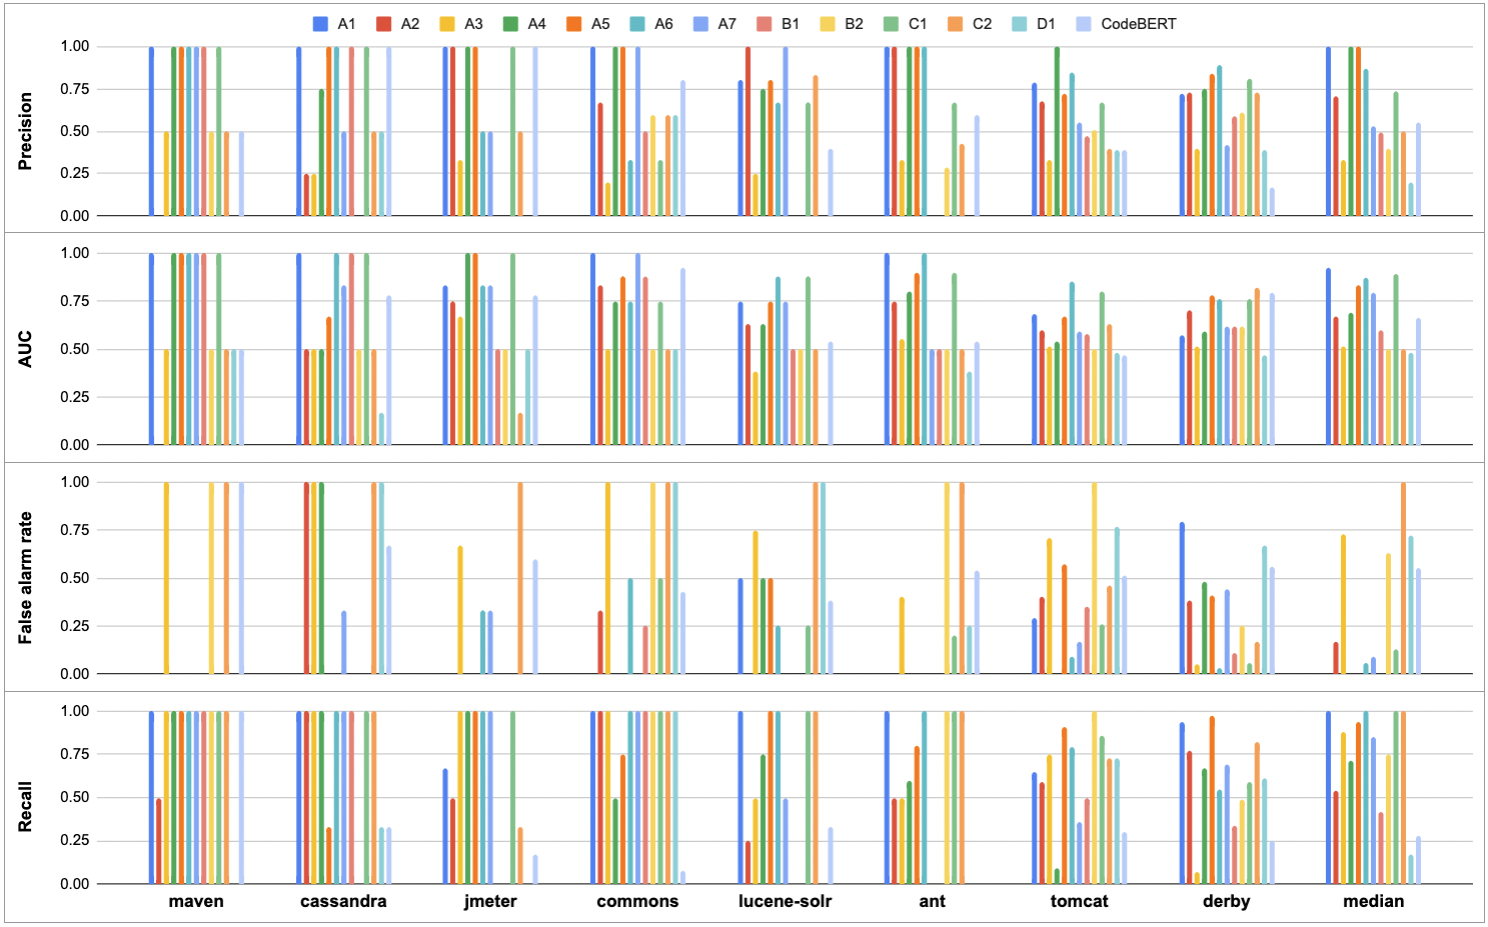
\includegraphics[width=\linewidth]{rahul/results.png}
%     \caption{Results of the ablation study (and for a  partial summary of these results, see Table~\ref{summary}).
%     The treatments A1,A2,A3,A4,A5,A6,A7,B1,B2,C1,C2,D1,Codebert are defined in Table~\ref{tab:treatments}.
%     Each treatment is
%     assessed using the metrics defined in
%     Table~\ref{tab:metrics}. Data sets are ordered left to right, smallest to largest (for details, see Table~\ref{tab:data}).
%       Median results shown on the right-hand-side.  }
%     \label{fig:results}
% \end{figure*}

\newcommand{\best}{\cellcolor{lightgray}}
\newcommand{\bad}{\cellcolor{pink}}

\begin{table*}[t]
\renewcommand{\baselinestretch}{.5}
{ 
   
    \caption{Our results across eight datasets on four metrics.}
    \label{tab:results}
   \scriptsize

    \begin{center}
    \begin{tabular}{l|llllllll|l}
    
        \toprule   
        \textbf{Treatment} & \textbf{maven} & \textbf{cassandra} & \textbf{jmeter} & \textbf{commons} & \textbf{lucene-solr} & \textbf{ant} & \textbf{tomcat} & \textbf{derby} & \textbf{median} \\
        \midrule
        \multicolumn{10}{c}{PRECISION  ({\em better} results are {\em larger})} \\
        \midrule
A1                      & 1   & 1    & 1    & 1    & 0.8  & 1    & 0.79 & 0.72 & 1             \\
A2                      & \bad 0   & \bad 0.25 & 1    & \bad 0.67 & 1    & 1    & \bad 0.68 & 0.73 & \bad 0.71          \\
A3                      & \bad 0.5 & \bad 0.25 & \bad 0.33 & \bad 0.2  & \bad 0.25 & \bad 0.33 & \bad 0.33 & \bad 0.4  & \bad 0.33          \\
A4                      & 1   & 0.75 & 1    & 1    & 0.75 & 1    & 1    & 0.75 & 1             \\
A5                      & 1   & 1    & 1    & 1    & 0.8  & 1    & 0.72 & 0.84 & 1             \\
A6                      & 1   & 1    & \bad 0.5  & \bad 0.33 & \bad 0.67 & 1    & 0.85 & 0.89 & 0.87 \\
A7                      & 1   & \bad 0.5  & \bad 0.5  & 1    & 1    & \bad 0    & \bad 0.55 & \bad 0.42 & \bad 0.53          \\
B1 (DODGE)              & 1   & 1    & \bad 0    & \bad 0.5  & \bad 0    & \bad 0    & \bad 0.47 & \bad 0.59 & \bad 0.49          \\
B2 (CNN)                & \bad 0.5 & \bad 0    & \bad 0    & \bad 0.6  & \bad 0    & \bad 0.29 & \bad 0.51 & \bad 0.61 & \bad 0.4           \\
C1 (DODGE)              & 1   & 1    & 1    & \bad 0.33 & \bad 0.67 & \bad 0.67 & \bad 0.67 & 0.81 & \bad 0.74          \\
C2 (CNN)                & \bad 0.5 & \bad 0.5  & \bad 0.5  & \bad 0.6  & 0.83 & \bad 0.43 & \bad 0.4  & 0.73 & \bad 0.5           \\
D1                      & \bad 0   & \bad 0.5  & \bad 0    & \bad 0.6  & \bad 0    & \bad 0    & \bad 0.39 & \bad 0.39 & \bad 0.2           \\
CodeBERT & \bad 0.5 & 1    & \bad 0.8    & \bad 0.63  & \bad 0.6  & \bad 0  & \bad 0.41 & \bad 0.25 & \bad 0.55 \\
    \midrule 
    \multicolumn{10}{c}{AUC: TP vs. TN ({\em better} results are {\em larger})}   \\
    \midrule
A1                   & 1   & 1    & 0.83 & 1    & 0.75 & 1    & 0.68 & 0.57 & 0.92          \\
A2                   & \bad 0   & \bad 0.5  & 0.75 & 0.83 & 0.63 & 0.75 & 0.6  & 0.7  & \bad 0.67          \\
A3                   & \bad 0.5 & \bad 0.5  & \bad 0.67 & \bad 0.5  & \bad 0.38 & \bad 0.55 & \bad 0.51 & 0.51 & \bad 0.51          \\
A4                   & 1   & 0.5  & 1    & 0.75 & 0.63 & 0.8  & 0.54 & 0.59 & 0.69          \\
A5                   & 1   & 0.67 & 1    & 0.88 & 0.75 & 0.9  & 0.67 & 0.78 & 0.83          \\
A6                   & 1   & 1    & 0.83 & 0.75 & 0.88 & 1    & 0.85 & 0.76 & 0.87 \\
A7                   & 1   & 0.83 & 0.83 & 1    & 0.75 & 0.5  & 0.59 & 0.62 & 0.79          \\
B1 (DODGE)           & 1   & 1    & 0.5  & 0.88 & 0.5  & 0.5  & 0.58 & 0.62 & 0.6           \\
B2 (CNN)             & \bad 0.5 & \bad 0.5  & \bad 0.5  & \bad 0.5  & \bad 0.5  & \bad 0.5  & \bad 0.5  & 0.62 & \bad 0.5           \\
C1 (DODGE)           & 1   & 1    & 1    & 0.75 & 0.88 & 0.9  & 0.8  & 0.76 & 0.89          \\
C2 (CNN)             & \bad 0.5 & \bad 0.5  & \bad 0.17 & \bad 0.5  & \bad 0.5  & \bad 0.5  & 0.63 & 0.82 & \bad 0.5           \\
D1                   & \bad 0.5 & \bad 0.17 & \bad 0.5  & \bad 0.5  & \bad 0    & \bad 0.38 & \bad 0.48 & \bad 0.47 & \bad 0.48          \\
CodeBERT & \bad 0.5 & \bad 0.56 & \bad 0.68 & \bad 0.53 & \bad 0.63 & \bad 0.48 & \bad 0.44 & 0.63 & \bad 0.54 \\
    \midrule
    \multicolumn{10}{c}{FALSE ALARM RATE ({\em better} results are {\em smaller})} \\
    \midrule
A1                     & 0 & 0    & 0    & 0    & 0.5  & 0    & 0.29 & 0.79 & 0             \\
A2                     & 0 & 1    & 0    & 0.33 & 0    & 0    & 0.4  & 0.38 & 0.17          \\
A3                     & \bad 1 & \bad 1    & \bad 0.67 & \bad 1    & \bad 0.75 & \bad 0.4  & \bad 0.71 & 0.05 & \bad 0.73          \\
A4                     & 0 & 1    & 0    & 0    & 0.5  & 0    & 0    & 0.48 & 0             \\
A5                     & 0 & 0    & 0    & 0    & 0.5  & 0    & 0.57 & 0.41 & 0             \\
A6                     & 0 & 0    & 0.33 & 0.5  & 0.25 & 0    & 0.09 & 0.03 & 0.06 \\
A7                     & 0 & 0.33 & 0.33 & 0    & 0    & 0    & 0.17 & 0.44 & 0.09          \\
B1 (DODGE)             & 0 & 0    & 0    & 0.25 & 0    & 0    & 0.35 & 0.11 & 0             \\
B2 (CNN)               & \bad 1 & 0    & 0    & \bad 1    & 0    & \bad 1    & \bad 1    & 0.25 & \bad 0.63          \\
C1 (DODGE)             & 0 & 0    & 0    & 0.5  & 0.25 & 0.2  & 0.26 & 0.06 & 0.13          \\
C2 (CNN)               & \bad 1 & \bad 1    & \bad 1    & \bad 1    & \bad 1    & \bad 1    & 0.46 & 0.17 & \bad 1             \\
D1                     & 0 & \bad 1    & 0    & \bad 1    & \bad 1    & \bad 0.25 & \bad 0.77 & \bad 0.67 & \bad 0.72          \\
CodeBERT & \bad 1 & 0 & \bad 0.2  & \bad 1 & 0.25 & \bad 0 &  0.28 &  0.17 & \bad 0.23\\
    \midrule
    \multicolumn{10}{c}{RECALL  ({\em better} results are {\em larger})} \\
    \midrule
A1                     & 1   & 1    & 0.67 & 1    & 1    & 1   & 0.65 & 0.94 & 1 \\
A2                     & \bad 0.5 & 1    & \bad 0.5  & 1    & \bad 0.25 & \bad 0.5 & 0.59 & \bad 0.77 & \bad 0.54       \\
A3                     & 1   & 1    & 1    & 1    & 0.5  & 0.5 & 0.75 & 0.07 & 0.88       \\
A4                     & 1   & 1    & 1    & \bad 0.5  & \bad 0.75 & \bad 0.6 & \bad 0.09 & \bad 0.67 & \bad 0.71       \\
A5                     & 1   & \bad 0.33 & 1    & \bad 0.75 & 1    & \bad 0.8 & 0.91 & 0.97 & 0.94       \\
A6                     & 1   & 1    & 1    & 1    & 1    & 1   & 0.79 & 0.55 & 1 \\
A7                     & 1   & 1    & 1    & 1    & 0.5  & 0   & 0.36 & 0.69 & 0.85       \\
B1 (DODGE)             & 1   & 1    & \bad 0    & 1    & \bad 0    & \bad 0   & \bad 0.5  & \bad 0.34 & \bad 0.42       \\
B2 (CNN)               & 1   & 0    & 0    & 1    & 0    & 1   & 1    & 0.49 & 0.75       \\
C1 (DODGE)             & 1   & 1    & 1    & 1    & 1    & 1   & 0.86 & 0.59 & 1          \\
C2 (CNN)               & 1   & 1    & 0.33 & 1    & 1    & 1   & 0.73 & 0.82 & 1 \\
D1                     & \bad 0   & \bad 0.33 & \bad 0    & 1    & \bad 0    & \bad 0   & \bad 0.73 & \bad 0.61 & \bad 0.17       \\
CodeBERT & 1   & \bad 0.33 & 0.67 &  1 & \bad 0.5 & \bad 0   & \bad 0.26  & \bad 0.25 &  \bad 0.42 \\
    \bottomrule
    \end{tabular}
    \end{center}
}
\end{table*}
 


As to the specifics of the other treatments:
\bi
\item
Treatment A5 is the treatments from the TSE'21 paper  that   proposed GHOSTing~\cite{yedida2021value}.
\item Treatment D1 contains the treatments applied in prior papers by   Yang et al.~\cite{yang2021learning}  and Kang et al. ~\cite{kang2022detecting}.
\item Anytime we applied {\em parameter engineering},
this meant that some automatic algorithm (DODGE) selected the control parameters for the learners (otherwise, we just used the default off-the-shelf settings). 
\item Anytime we apply {\em label engineering}, we are only
used 10\% of the labels in the training data.
\item The last line, showing CodeBERT, has no pre-processing or tuning. As said   above, CodeBERT is so complex that we must  run it ``off-the-shelf''.
\ei

 
% We now discuss our updated approach, which we recommend. We start by combining the train and test set data. We split this data 80/20 into train and test sets (exception: for maven, we split 50/50, since there are only 4 samples in total). We discard all non-numeric columns. We set the ``closed'' label to 1 and the ``open'' label to 0. This is because in doing this, the class imbalance ratio is below 0.5, which is in agreement with the original domain of GHOST (defect prediction). Indeed, by setting the labels to the reverse, our results were worse. This is not by coincidence: because we followed the GHOST algorithm from \citet{yedida2021value}, we also ended up using their weighted loss function. Such a loss function is inherently asymmetric, making the two learning problems (with each set of labels) different, one more difficult than the other.


% At this point, we use SMOTE (i.e., instance engineering), followed by two rounds of fuzzy sampling (boundary engineering) and then SMOTE again. Note that the process of using two rounds of fuzzy sampling followed by SMOTE was recommended by the original GHOST paper Finally, we use DODGE to optimize the number of layers and the number of units per layer in a feedforward network. In essence, our approach is GHOST with the addition of label engineering (and the additional SMOTE step).

% \subsection{Fuzzy sampling and $\beta-$smoothness}

% \begin{figure*}[t]
%     \centering
%     \begin{subfigure}{.49\linewidth}
%         \centering
%         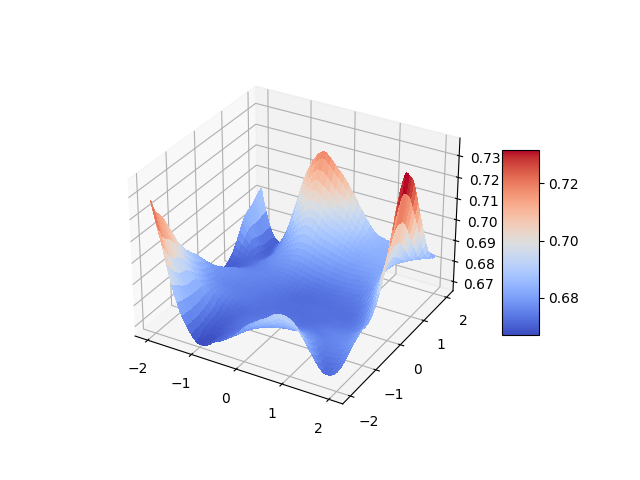
\includegraphics[width=\textwidth]{rahul/tomcat-pre.png}
%         \caption{Before fuzzy sampling}
%     \end{subfigure}
%     \begin{subfigure}{.49\linewidth}
%         \centering
%         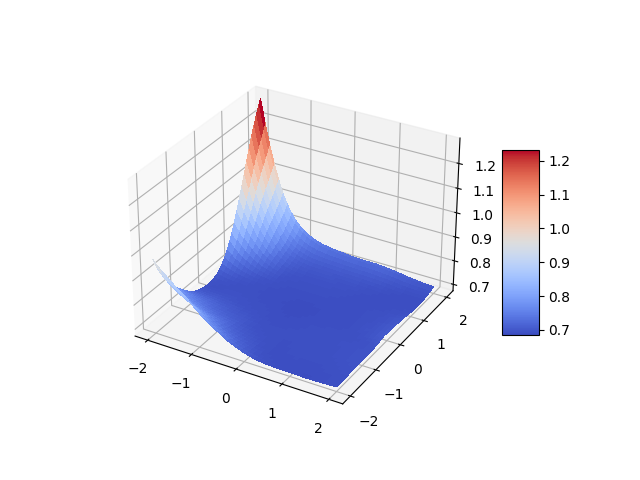
\includegraphics[width=\textwidth]{rahul/tomcat-post.png}
%         \caption{After fuzzy sampling}
%     \end{subfigure}
%     \caption{Loss landscape surface (a) before and (b) after fuzzy sampling.}
%     \label{fig:loss}
% \end{figure*}

% We prove here that fuzzy sampling improves the smoothness of the loss function, making optimization easier. We begin by using the approach of \citet{li2018visualizing} to visualize the loss landscapes before and after using fuzzy sampling. Figure \ref{fig:loss} shows the results of this on the tomcat dataset. Notice that after using fuzzy sampling, the loss surface is significantly smoother. We notice this pattern continue across all our datasets.

% Next, we formalize this notion of smoothness. Recall that the $\beta-$smoothness is defined as the maximum value of $\beta$ for which $\lVert \nabla f(x_1) - \nabla f(x_2) \rVert \leq \beta \lVert x_1 - x_2 \rVert$ under some norm (we use the $l_2$ norm), and is a measure of the smoothness of the loss surface (i.e., higher the $\beta-$smoothness, smoother the loss surface). This is merely the gradient of the Lipschitz constant, which for the binary cross-entropy loss, \citet{yedida2021lipschitzlr} derived as

% \[
%     \frac{\partial^2 \mathcal{L}}{\partial w^{[L]2}_{ij}} = \frac{1}{m} g(\boldsymbol z^{[L]}) (1 - g(\boldsymbol z^{[L]})) a^{[L-1]}_j
% \]

% (here, $\mathcal{L}$ is the loss function, $\boldsymbol w^{[L]}$ is the weight matrix at layer $L$, $L$ is the number of layers, $m$ is the number of training examples in a batch, $g$ is the activation function (at layer $L$, this is the sigmoid function), $\boldsymbol a^{[L-1]}$ is the activation vector at layer $L-1$, and $\boldsymbol z^{[L]}$ is the pre-activation vector, $\boldsymbol z^{[L]} = \boldsymbol W^{[L]T} a^{[L-1]} + b^{[L]}$ for bias vector $b^{[L]}$)

% \begin{table}[h]
%     \centering
%     \caption{Percent changes in the $\beta-$smoothness after fuzzy sampling.}
%     \label{tab:fuzzy}
%     \begin{tabular}{ll}
%         \toprule
%         \textbf{Dataset} & \textbf{\% change} \\
%         \midrule
%         ant & 24.78 \\
%         cassandra & 73.09 \\
%         commons & 29.61 \\
%         derby & 31.35 \\
%         jmeter & 55.53 \\
%         lucene-solr & 16.46 \\
%         maven & 158.87 \\
%         tomcat & 36.34 \\
%         \midrule
%         \textbf{median} & \textbf{33.85} \\
%         \bottomrule
%     \end{tabular}
% \end{table}

% $a^{[L-1]}_j$ is a constant with respect to $\boldsymbol w^{[L]}_{ij}$; for the others, it is trivial to show that an extremum occurs at $\boldsymbol z^{[L]} = 0$, so that $g(\boldsymbol z^{[L]}) = \frac{1}{2}$. Therefore, the $\beta-$smoothness is

% \[
%     \beta = \frac{1}{4m} \max\limits_j \Vert a_j^{[L-1]} \rVert
% \]  

% Because the numerator needs to be computed experimentally, we use this equation to compute the $\beta-$smoothness of the loss surface for each dataset before and after fuzzy sampling. Table \ref{tab:fuzzy} shows the percent changes of the $\beta-$smoothness after using fuzzy sampling. For all datasets, this percent change is positive and significant. Finally, we note that the $\beta-$smoothness is independent of the labels, so the gains from label engineering are independent of the gains from fuzzy sampling.


\section{Results}
\label{sec:results}




\newcommand{\ans}[1]{\underline{\textbf{Answer~#1:}}}


 
 
  \begin{table} 
  \caption{Median performance improvements seen after applying all the treatments A1 (defined in \S\ref{rx}); i.e. all of
{\em instance}, {\em label}, {\em boundary}  and {\em parameter} engineering.}
 \begin{center}
{\scriptsize  \begin{tabular}{|c|c|c|c|c|}\cline{3-5} 
    \multicolumn{2}{c|}{} &       &  From right-& \\ 
    \multicolumn{2}{c|}{} & From     &  hand-side & \\  
     \multicolumn{2}{c|}{} &   Table~\ref{tab:initial_svm}  &  of Table~\ref{tab:results} &  Improvement \\\hline
                             & precision   & 50 & 100 & 50\\ 
{\em higher} is {\em better} & AUC         &  41& 90 & 59\\ 
                             & recall      &  19 & 100 & 89\\\hline
{\em lower} is {\em better}  & false alarm & 32 & 0 & 32\\\hline
\end{tabular}} 
\end{center}
\label{summary}
\end{table}
  
  
  
 

% Given the large improvements seen after apply our treta  large improvements seen in Table~\ref{summary} conjectured that learners fault to predict actionable
% static code warnings if they must negotiate a complex decision landscape. 

% o remove the ``bumpiness'' in data like Figure~\ref{fig:loss}, we need to 
% pull and push the decision boundaries between different classes into a smoother shape.
% But also, unlike simplistic $(C,\gamma)$ tuning available in radial  SVMs, we want that process to perform differently
% in different parts of the data.


The results of the Table~\ref{tab:treatments} treatments are shown in   Table~\ref{tab:results}
(and 
another brief summary is offered in
Table~\ref{summary}).
These results are somewhat
extensive
  so, by way of an overview, we offer the following summary tool.
 The cells shown in  \colorbox{pink}{pink} are those that are   worse than the A1 results 
  (and A1 is our recommended GHOST2 method). 
 Looking over those pink cells
 we can see that across our data sets and across our different measures, our recommend method (A1) does as well (or better) than anything else. 
 
 (Technical aside: looking at this pink cells, it could be said that   A5 comes close to A1, but A5 loses a little on recalls).
 Nevertheless, we have strong reasons for recommending A1 over A5 since, recalling Table~\ref{tab:treatments},
 A5 requires a labelling for 100\% of the data. On the other hand A1, that uses label engineering,
 achieves its results using 10\% of the labels. This is important since, as  said in our introduction, 
one way to address, in part, the methodological problems
raised by Kang et al. GHOST2 makes its conclusions
using a small percentage of the raw data (10\%). That is,
to address to issues of corrupt data found by Kang et
al., we say ``use less data'' and, for the data that is used,
``reflect more on that data''.)
 
 Using these results,
we can answer our research questions as follows. 
 


\subsection*{ \rqn{1} For detecting actionable static code warnings,
what data mining methods should we recommend?}
  

Regarding feedforward networks versus, say,  traditional learners (decision trees, random forests, logistic regression and SVMs), the traditional learners all performed worse than the 
feedforward networks used in treatment A1 (evidence: compare treatments
A1 with A7 which use feedforward or traditional learners, respectively; there are four perfect AUCs
for feedforward networks in A1, i.e AUC=100\%, but only two for the A7 results). 



As to why 
the 1980s style
feedforward networks worked better than newer neural net technology,  we note that feedforward networks run so fast
than it is easier to extensively tune them. Perhaps
 (a)~faster learning plus (b)~more tuning might lead to better results
that then non-linear modeling of an off-the-shelf learner.
This could be an interesting avenue for future work.

As to the value of {\em boundary, label, instance}
and {\em parameter} engineering,   in the ablation study, removing any of these led to worse results.
For example, 
with {\em boundary engineering},
   A1
(that uses boundary engineering) generates more perfect
scores (e.g. AUC=100\%) than A4 (that does not use it).
Also, for recall, A1 always performed
as good or better than A4 in 6/8 data sets. Similarly, A4 suffers from a drop in AUC score across the board.

 
As for {\em label engineering}, from A1 to A5,
specializing our data to just 10\% of
the labels (in A1) yields nearly the same precisions
which using 100\% of the data (in A5) in nearly all the AUC results. Moreover, the AUC score for A1 is perfect in 4/8 cases, while for A5, it is rarely the case.



As to {\em instance engineering},
without it the  
precision can crash to zero
(compare A1 to A2, particularly  the smaller data sets) while often leading to
lower recalls. The smaller datasets also see a decrease in AUC for A2.


 
Measured in terms of false alarm, these results strongly recommend 
{\em parameter engineering}. Without parameter engineering, some of those treatments could find too many static code warnings and hence suffer from
excessive false alarms (evidence: see the A3 false alarm results in nearly every data set). A1 (which used all the   treatments of \S\ref{rx}) had lower false alarm rates than anything else (evidence: we rarely see the dark blue A1 spike in the false alarm results). The  only exception to the observation that ``parameter engineering leads to lower false alarm results''
are seen in the   DERBY
data set. That data set turns out to be particularly tricky in that, nearly always, modeling methods  that achieved low false alarm rates on that data set
also had to be satisfied with much lower recalls. 
 
 
\begin{figure}[!t]
   \begin{center}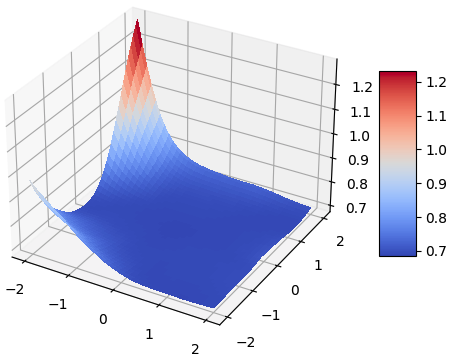
\includegraphics[width=.3\textwidth]{rahul/after.png} \end{center} 
    \caption{ Error landscape in the TOMCAT  after applying the treatments of \S\ref{rx}. To understand the simplifications achieved via our methods, the reader might find it insightful to  compare this figure against Figure~\ref{fig:loss}. }
    \label{fig:gain}
\end{figure}



One final point is that these results do not  recommend 
the use of certain widely used neural network
technologies such as CNN or CodeBERT for finding actionable
static code warnings.
CNN-based treatments (B2 and C2) suffer from low precision and AUC scores (see Table \ref{tab:results}).
Similarly, as shown Table~\ref{tab:results}, CodeBERT
often suffers from   low precision and poor false alarms
and (in the case of CodeBERT) some very low recalls indeed.


In summary:
\begin{formal}
\ans{1} To recognize actionable static code warnings, apply all the treatments of \S\ref{rx}. Also, 
spend most tuning faster feedforward neural nets  rather than trusting (a)~traditional learners or (b)~more recent
``bleeding edge'' neural net methods.
\end{formal}



  
 
\subsection*{\rqn{2} Does GHOST2's combination of instance, label, boundary
and parameter engineering, reduce the complexity of the
decision boundary?}

Previously, this paper argued
that reason for the poor performance
seen in prior was due to the complexity
of the data (specifically, the bumpy shape seen in  Figure~\ref{fig:loss}).
Our treatments of \S\ref{rx} were  designed to simplify that landscape. Did we succeed?

 Figure~\ref{fig:gain}
 shows the landscape in  TOMCAT after
 the   treatments of \S\ref{rx}
 were applied.
 By comparing this figure with
      Figure~\ref{fig:loss},
      we can see that our treatments
      achieved the desired goal
      of removing the ``bumps''.
      
 
 \begin{wraptable}{r}{1.7in}
     
    \caption{Percent changes in \citet{li2018visualizing}'s
    smoothness metric, seem after applying the methods of this paper.}
    \label{tab:fuzzy}
    \begin{tabular}{lr}
        \toprule
        \textbf{Dataset} & \textbf{\% change} \\
        \midrule
        
   \rowcolor{gray!15}       maven & 158.87 \\
        
        cassandra & 73.09 \\
        
        \rowcolor{gray!15}       jmeter & 55.53 \\
        tomcat & 36.34 \\
        \rowcolor{gray!15}       derby & 31.35 \\
        commons & 29.61 \\
         \rowcolor{gray!15}      ant & 24.78 \\
        lucene-solr & 16.46 \\
        \midrule
        \textbf{median} & \textbf{33.85} \\
        \bottomrule
    \end{tabular}
\end{wraptable}

 As to the other data
      sets,
      \citet{li2018visualizing}
      propose a ``smoothness'' equation
      to measure a data set's
      ``bumps''.
      Table~\ref{tab:fuzzy}
      shows the percentage 
      change in that smoothness
      measure seen   after applying the methods of this paper. 
       All these changes
    are positive, indicating that the resulting landscapes are much smoother.
    For an intuition of what these numbers mean,    the TOMCAT change of 36.35\% results in Figure \ref{fig:loss}  
    changing to Figure \ref{fig:gain}.
    
    Hence we say:
    
    
\begin{formal}
\ans{2} Label, parameter, instance and boundary engineering can simplify the
internal structure of   training
data.
\end{formal}





\subsection*{
\rqn{3}  Does  GHOST2's  combination of {\em instance}, {\em label}, {\em boundary}  and {\em parameter}  improve predictive performance?} 
     
   
 Table~\ref{summary} shows the performance
 improvements   after
 smoothing out our training
 data from (e.g.)
 Figure \ref{fig:loss} to 
 Figure \ref{fig:gain}. On 4/8 datasets, we achieve perfect scores. Moreover, we showed through an ablation study that each of the components of GHOST2 is necessary. For example, row A3 in Table \ref{tab:results} is another piece of evidence that hyper-parameter optimization is necessary. The feedforward networks of our approach outperformed more complex learners (CNNs and CodeBERT)--we refer the reader to rows B2, C2, and CodeBERT in Table \ref{tab:results}. On the other hand, going too simple for traditional learners leads to A7, which suffers from poor precision scores.
 Given those large improvements, we say: 
 
\begin{formal}
\ans{3} 
Detectors of actionable 
 static code warnings  work much better 
 when learned from smoothed
 training data.
 \end{formal}
 
 


\subsection*{  
\rqn{4}  Are all parts of GHOST2 necessary; i.e. would
something simpler also achieve the overall goal?}

We presented an ablation study that showed that each part of GHOST2 was necessary. Among the 13 treatments that we tested, GHOST2 was the only one that consistently scored highly in precision, AUC, and recall, while also generally having low false alarm rates. The crux of our ablation study was that each component of GHOST2 works with the others to produce a strong performer.
 
 Based on the above ablation study results, we say:
 \begin{formal}
\ans{4} Ignoring any of
part of
instance,  label,  boundary  or parameter engineering leads to worse results than
using all parts (at least for the purpose of recognizing actionable static code
warnings).
\end{formal}



 \subsection*{
\rqn{5}  Are larger training sets necessary (for the task of recognizing actionable static code warnings)?}
 
 In the above discussion, when we presented
Table~\ref{tab:data}, it was noted that several
of the train/tests used in this study were very small. At that time, we expressed a concern that, possibly, our   data sets explored   were too small for effective learning. 


This turned out not to be the case.
Recall that in 
  Table~\ref{tab:results},
  the data set were sorted left-to-right from smallest to largest training set size. There is no pattern there  that smaller data sets perform worse than large ones.  In fact-- quite the opposite: the smaller data sets were always associated with better performance than those seen on right-left-side.  Hence we say:
  
  
  \begin{formal}
\ans{5} The methods of this paper are effective,
even for very small data sets.
\end{formal}


This is a surprising result since one of the truisms of data mining is ``the more data the better''. 
 Large data sets  are often cited as the key to success for data
mining applications. For example, in his famous talk, ``The
Unreasonable Effectiveness of Data'',
Google’s former Chief Scientist
Peter Norvig argues that ``billions of trivial data points can
lead to understanding''~\cite{norvig11} (a claim he supports with numerous
examples from vision research).



 
%  \noindent
% \rqn{6} \textit{For our task, what at the cost and benefits of different kinds of neural learners?}
 

%  \begin{formal}
% \ans{6}XXX
% \end{formal}


% \noindent
% \rqn{7} \textit{Are larger training sets useful (for this task)?}



%  \begin{formal}
% \ans{7}XXX
% \end{formal}
% \bi
 
% \item
% \underline{\bf RQ3}: {\em Does this   combination of methods achieve the desired effect?}
%  Figure \ref{fig:loss}b shows the TOMCAT error landscape in our training data {\em after} applying   {\em instance} engineering, {\em label} engineering, {\em boundary} engineering and {\em parameter engineering}. Note that this landscape is far smoother than that seen in  Figure \ref{fig:loss}a.
%  This pattern (that our methods smoothed the loss landscape) was also seen in all our other data (see Table~\ref{fuzzy}).
% \item
% \underline{\bf RQ4}: {\em Does this desired effect achieve the overall goal?} As will be shown by the experimental section of this paper, defectors of static code warning false alarms work much better in our smoother data spaces, and out-perform (by a large margin) the results of Table~\cite{initial_svm}.
% \ei
% (Note that, later in this paper, we will add other research questions.)


% Note that 
% ``A1`` uses our simplest neural network (feedforward networks) since (a)~tuning very fast feedforward networks is much faster than tuning slower CNN algorithms; and (b)~our results did not show  that
% CNN out-performing feedforward networks.

% We recognize that the fuzzy sampling technique combined with hyper-parameter optimization yielded excellent results in the original GHOST study. Therefore, this approach is employed with classical learners. Here, we obtain excellent results (median AUC=1.0, see treatment A6). However, the data used in this study, which was provided by \citet{kang2022detecting}, was manually labeled, which is an expensive task. We therefore ask if this labeling is inherently necessary.

 




% \citet{yang2021learning} suggested that the low intrinsic dimensionality of the datasets used in their study meant that recognizing actionable static code warnings was an intrinsically easy task. This led to them using SVMs for their work. Given that the dataset was disputed and corrected by \citet{kang2022detecting}, we test if that assumption still holds. Specifically, we ask if complex deep learners
% are needed for this task, or would simpler learners suffice?

% \rqn{2} \textit{Can deep learning help recognize actionable static code warnings?}

% The work of \citet{kang2022detecting} showed that the SVM methods of \citet{yang2021learning} were no longer sufficient for the task. We show that this is indeed true, as part of an ablation study. We further show that in fact, classical learners are insufficient for the task, even with hyper-parameter optimization \cite{agrawal2019dodge,menzies2018500+} and SMOTE (see treatment C1 in our ablation study, Table \ref{tab:treatments}). Therefore, we turn to deep learning, but begin by exploring the simplest deep learning model, the feedforward network. Motivated by a recent success in defect prediction \cite{yedida2021value}, we try the GHOST algorithm, which combines feedforward networks with hyper-parameter optimization and a novel fuzzy sampling approach. However, this falls short of our expectations (see treatment A5 from our ablation study). Moreover, the use of more complex deep learners such as CNNs (see treatments B2 and C2), and CodeBERT (see the last line of Table \ref{tab:treatments}) were also insufficient. These disappointments lead to our next research question:

% \rqn{3} \textit{How can we recognize actionable static code warnings?}

% We recognize that the fuzzy sampling technique combined with hyper-parameter optimization yielded excellent results in the original GHOST study. Therefore, this approach is employed with classical learners. Here, we obtain excellent results (median AUC=1.0, see treatment A6). However, the data used in this study, which was provided by \citet{kang2022detecting}, was manually labeled, which is an expensive task. We therefore ask if this labeling is inherently necessary.

% \rqn{4} \textit{Can we recognize actionable static code warnings with fewer labels?}

% In this RQ, we explore the problem under the semi-supervised setting. Consequently, we develop a novel yet trivial semi-supervised algorithm that provides labels to samples that do not have any. In doing so, we can still achieve excellent results (median AUC=0.88), while using only 9.5\% labels. Moreover, looking closely at this result (see A1 in our ablation study) and A6, we see that the IoU of the median performance (intersection over union, an extension of Jaccard similarity) is 0.67. More interestingly, however, we observe a small data result, where our recommended approach (A1, which we call GHOST2) performs well on datasets with few samples, and worse on larger datasets. Therefore, we ask:

% \rqn{5} \textit{Are neural networks practical on small datasets in SE?}

% While we can only provide an answer about our specific problem, this opens up a larger discussion about truisms of deep learning that do not hold up in software engineering. Specifically, our results challenge the notion that deep learning requires large amounts of data to work well; instead, we say that for simpler problems like in SE, neural networks can achieve excellent results using less data. Finally, we ask:

% \rqn{6} \textit{What lessons can practitioners learn from our results?}

% We notice that our work provides yet another case study where using AI tools off-the-shelf does not work. Specifically, we characterize a learning problem as a set of engineering decisions: boundary engineering, label engineering, learner choice, hyper-parameter engineering, and instance engineering. We recommend that practitioners rethink learning problems as these different challenges and use a combination of tools that works for their problem from these different areas.

% \rqn{7} \textit{How does fuzzy sampling help optimization?}

% We seek to find why fuzzy sampling is so important to our approach. To do so, we show that using fuzzy sampling improves the $\beta-$smoothness of the loss surface, making it easier to optimize.


% Our results are shown in Figure \ref{fig:results}. A1 is our recommended approach, and uses 9.5\% of labels. Looking at the graphs, it is clear that A1 is the strongest contender. For example, against B1, A1 wins (or ties) in precision in all cases, and wins (or ties) in AUC in 7/8 datasets. In false alarm rate, A1 wins/ties 6/8 times, and in recall, it wins/ties 7/8 times. Meanwhile, the method recommended by the original study (SVMs with balanced class weights and normalizing), which is shown as D1, performs poorly across the board.

% More interesting than the comparison between the treatments, however, is a trend that can be seen with respect to dataset size. In Figure \ref{fig:results}, the datasets are sorted by size. In several cases, A1 loses to other treatments on derby and tomcat, the two largest datasets, while winning across the other datasets. For example, against A6, in both AUC and precision, A1 wins in all datasets except in derby and tomcat (on AUC, it also loses on lucene-solr). Similarly, on precision, A1 matches or outperforms A5 in all datasets except derby. This is perhaps a ``small data'' result where feedforward networks, i.e., neural approaches, outperform other approaches on small datasets, even though conventional wisdom is that more data is better for neural networks. Going deeper into A1 vs. A5, Table \ref{tab:treatments} shows that the difference between the two is that A5 does not use the semi-supervised learning. This could be the reason it does better on large data. In detail, when there is less data available, a neural network is susceptible to change its boundary more drastically with each training sample. When more samples are available, however, it must accommodate all of them, making changes to the decision boundary more subtle. Therefore, on small datasets, our semi-supervised learning technique has a regularization effect where by not trusting the labels given and instead using the nearest neighbors, we reduce the shift in the decision boundary. On larger datasets, however, this semi-supervised technique, where we modify the labels \textit{a priori}, has the negative effect of corrupting the data and confusing the learner. Our lesson from this is that for datasets with less than 30 training samples (which is all the datasets till and including ant), semi-supervised learning is advisable. 

% At this point, we digress to make a clarification. Although we explain the superiority of A5 in the larger datasets as a consequence of the effect of semi-supervised learning on the boundary, that does \textit{not} make it a boundary engineering technique; rather, the change in labels is the cause the boundary shifts. Our definition of boundary engineering covers changes to the \textit{independent variables} that affect the boundary, such as fuzzy sampling and kernel methods.

% We now discuss our results in the context of seven research questions:

% \rqn{1} \textit{Is recognizing static code warnings (still) intrinsically easy?}

% % \hl{Sherry}
% The intrinsic dimensionality of each project after applying a box-counting dimension reduction algorithm are summarized in in Table~\ref{tab:intrinsic}, and we sort the project in a ascending order of their intrinsic dimension. The results illustrate our datasets are still intrinsically easy.

% \begin{table}[]
% \caption{Summary of dimensionality of eight projects. The projects are sorted in the ascending order of their intrinsic dimensionality.}
% \label{tab:intrinsic}
% \begin{tabular}{llll}
% \toprule
% Project     & \begin{tabular}[c]{@{}l@{}}Original\\ Dimensionality\end{tabular} & \begin{tabular}[c]{@{}l@{}}Intrinsic\\ Dimensionality\end{tabular} & Instance number \\ \midrule
% commons     & 127                                                               & \textbf{3.45}                                                              & 22              \\ 
% derby       & 292                                                               & \textbf{3.45}                                                               & 458             \\ 
% tomcat      & 284                                                               & \textbf{3.64}                                                               & 184             \\ 
% lucene-solr & 278                                                               & 3.83                                                               & 30              \\ 
% ant         & 329                                                               & \textbf{4.62}                                                               & 35              \\ 
% cassandra   & 265                                                               & \textbf{5.47}                                                               & 17              \\ 
% maven       & 22                                                                & \textbf{5.47}                                                               & 4               \\ 
% jmeter      & 287                                                               & \textbf{5.79}                                                               & 18              \\
% \bottomrule
% \end{tabular}
% \end{table}

% \rqn{2} \textit{Can deep learning help recognize static code warnings?}

% Our results with A5 (GHOST), B2 and C2 (CNNs), and CodeBERT show that deep learners cannot be used as-is for detecting actionable static code warnings. Indeed, their performance leaves more to be desired. Our conclusion is:

% \begin{formal}
%     \noindent
%     Deep learning cannot be used as-is for recognizing static code warnings.
% \end{formal}

% \rqn{3} \textit{How can we recognize static code warnings?}

% We showed that using a combination of engineering techniques, leading up to one of our recommendations (A5) worked well to recognize actionable static code warnings. While it uses all the labels, it is fast and computationally cheap.

% \begin{formal}
%     \noindent
%     A combination of engineering techniques such as boundary engineering, learner choice, and hyper-parameter engineering can work together to achieve strong results.
% \end{formal}

% \rqn{4} \textit{Can we recognize static code warnings with fewer labels?}

% Our label engineering method allows us to achieve strong results using just 9.5\% of labels on average. It is certainly possible that better semi-supervised learning techniques might produce better results; however, we do not explore that in this paper.

% \begin{formal}
%     \noindent
%     Semi-supervised learning can help achieve strong results using only 9.5\% of labels.
% \end{formal}

% \rqn{5} \textit{Are neural networks practical on small datasets in SE?}

% Our results with A1 (GHOST2) show that neural approaches are certainly practical and useful for achieving high performance on small datasets, even as low as 4 samples (in the case of maven). Therefore, we say:

% \begin{formal}
%     \noindent
%     At least in SE, neural networks are practical on small data.
% \end{formal}

% We also comment here that as shown by \citet{zhang2017understanding}, neural networks are often \textit{over-parameterized}, i.e. they have more parameters than data samples. This is not a problem: \citet{du2018gradient} show that stochastic gradient descent can optimize such networks. We believe this is one of the reasons that our feedforward networks worked for small datasets. Our larger models had trouble with hyper-parameter optimization. For CNNs, we experienced frequent crashes for unknown reasons. CodeBERT was too slow for hyper-parameter optimization, and we did not attempt it. These models, while over-parameterized, have \textit{too many} parameters, making optimization too slow for tuning (CNNs, for example had $\mathcal{O}(10^5)$ parameters, while feedforward networks had $\mathcal{O}(10^3)$ parameters). We therefore conjecture that there is thus a ``Goldilocks effect'' in place, where classical learners may not have the representation power (too few parameters), deep learners like CodeBERT have too many parameters to optimize, and feedforward networks are ``just right''. We leave further exploration of this to future work.

% \rqn{6} \textit{How does fuzzy sampling help optimization?}

% To understand this, we took inspiration from a seminal paper that explained how batch normalization helps optimization \cite{santurkar2018does}. In that paper, they showed that batch normalization improved the $\beta-$smoothness of the loss surface, making optimization easier. We use a similar approach. First, using the technique by \citet{li2018visualizing}, we showed that the loss surface is indeed, smoother. Next, we formalized the smoothness of the loss surface. We extended the work of \citet{yedida2021lipschitzlr}, who derived the Lipschitz constants of loss functions. Recalling that the $\beta-$smoothness is the maximum gradient of the Lipschitz constant, we used their equations of the Lipschitz constant to derive the $\beta-$smoothness. Finally, we implemented it and show that the smoothness is improved by a median of 33.85\%.

% \begin{formal}
%     \noindent
%     Fuzzy sampling helps smoothen the loss surface, making optimization easier.
% \end{formal}

% \rqn{7} \textit{What lessons can practitioners learn from our results?}

% We offer several lessons from our work:

% \begin{formal}
%     \be
%         \item Mistrust your data more. Labels may not always be accurate, and data can have errors.
%         \item Attempt to use fewer labels when possible to lower manual effort required to label data.
%         \item Our empirical methods may need to be revised for small data.
%         \item Do not use tools off-the-shelf; use hyper-parameter optimization and consider the engineering decisions of the problem carefully.
%         \item We learn from failures as well as successes. Work with your critics.
%     \ee
% \end{formal}

 
 \section{Threats to Validity}
\label{sec:threats}
 
 
 As with any empirical study, biases can affect the final results. Therefore, any conclusions made from this work must be considered with the following issues in mind: 
 
 {\em 1. Sampling bias } threatens any classification experiment; i.e., what matters there may not be true here. For example, the data sets used here comes prior work
 and, possibly, if we explored other data sets we might reach other conclusions.
On the other hand, {\em repeatability} is an important part of science so we argue
that our decision to use the Kang et al. data is appropriate and respectful to both that prior work
and the scientific method.   
 
 {\em 2. Learner bias:} Machine learning is a large and active field and any single study can only use a small subset of the known  algorithms. Our choice of ``local learning'' tools was explained in \S\ref{rx}. That said, it is important to repeat the comments made there
 that our SMOTEing, SMOOTHing, GHOSTing and DODGEing   operators
 are but one set of  choice within a larger framework of possible approaches to instance, label, boundary, and parameter engineering (respectively).
 As SE research matures, we foresee that our framework will become a workbench   within which researchers replace some/all of these treatments with better options. That said, in defence of the current options, we note that our ablation study showed that removing any of them can lead to worse results. 
 
 
 
 {\em 3. Parameter bias}: Learners are controlled by parameters and the resulting performance can change dramatically if those parameters are changed. Accordingly,
 in this paper, our recommended methods (from Table~\ref{rx}) includes parameter engineering methods to find good parameter settings for our different data sets.  
 
 
 {\em 4. Evaluation bias:} This paper use four evaluation criteria (precision, AUC, false alarm rate, and recall) and it is certainly true that by other measures, our results might not work be seen to work as as well. In defence of our current selection, we note that we use these measures since they let us compare our new results to prior work (who reported their results using the same measures).
 
 Also, to repeat a remark made previously, another evaluation bias was how we separated data into train/test.  In other papers, we have run repeated
trials with multiple 80:20 splits for training:test data. This
was not here since some of our data sets are too small (see
the first few rows of Table 5) that any reduction in the
training set size might disadvantage the learning process.
Hence, the external validity claims of this paper come from
patterns seen in eight different software projects.
 
  

\section{Discussion}
\label{sec:discussion}

This discussion section steps back from the above to make some more general points.



We suggest that this paper should lead to a new way of training
newcomers in software analytics:
\bi
\item
Our results show that there is much value in decades-old learning technology
(feedforward networks). Hence, we say that when we train newcomers to the field of software analytics,
we should certainly train them in the latest techniques (deep learning, CodeBERT, etc).
\item
That said,
we should also ensure that they know of prior work since (as shown above), sometimes
those older methods still have currency. 
For example,
if some learner is faster to run, then it is easier to tune. 
Hence, as shown above, it can be possible for old techniques to do better than new ones, just by tuning.  
\ei
   For future work, it would be useful to check what other SE domains
    simpler, faster, learners  (plus some tuning)
   out-perform more complex learning methods.


That said, we offer the following cautionary note about tuning.
Hyper-parameter  optimization (HPO, which  we have call ``parameter engineering'' in this paper)
  has received much recent attention in the SE literature~\cite{agrawal2019dodge,yedida2021value,agrawal2021simpler} 
We have shown here that reliance on {\em just} HPO can be foolhardy
since better results can be obtained by the 
judicious  use of HPO combined with more nuanced approaches that actually reflect the particulars of the
current problem (e.g. our treatments that adjusted different parts of the data in different ways).
As to how much to study the internals of a learner,
we showed above  that there are many choices deep within a learner than can greatly improve predictive performance.  Hence we say that it   is very important to know the internals of a learner and how to adjust them.
In our opinion, all too often, software engineers use AI tools as ``black boxes'' with little
understanding of their internal structure. 

Our results also  doubt some of the truisms of our field. 
For example:
\bi
\item There is much recent work on big data research in SE, the premise being that ``the more data, the better''. We certainly do not dispute that but
our  results do show that it is possible to achieve good results with very small data sets.
\item
There is much work in software analytics suggesting that  deep learning is a superior method for analyzing data \cite{yedida2021value, wang2018deep, li2017cclearner, white2015deep}. Yet when we tried that here, we found that a decades-old neural net architecture (feed-forward networks, discussed in Table \ref{tab:nnhere}) significantly out-performed deep learners. 
\ei
For newcomers to the field of software analytics,
truisms   might be useful. But better results
might be obtained when teams of data scientists
combine to suggest  multiple techniques-- some of which ignore supposedly tried-and-true truisms.
  
 
  
  
\section{Conclusion}
\label{sec:conclusion}

Static analysis tools often
suffer from a large number of false alarms that are deemed
to be unactionable~\cite{tomassi2021real}. Hence, developers often ignore
many of their warnings. Prior work by 
Yang et al.~\cite{yang2021learning} attempted to build predictors for
actionable warnings but,
as shown by Kang et al.~\cite{kang2022detecting}, that study used
poorly labelled data. 

This paper extends the  Kang et al. result as follows.
 Table~\ref{tab:initial_svm} shows that building
 models for this domain is a challenging task. 
 The discussion section of \S\ref{problem}
 conjectured that for the purposes of detecting
 actionable static code warnings, standard
 data miners can not handle the complexities of
 the   decision boundary. More specifically, 
 we argued that:
 \begin{quote}
 {\em 
 For complex data, \underline{\bf global} treatments  
   perform worse  than \underline{\bf localized} treatments
 which   adjust different parts of the  landscape in 
 different ways.}
 \end{quote}
 \S\ref{rx} proposed four such localized treatments, 
 which we called instance, parameter, label and boundary engineering.
 
 These treatments were tested on the data generated by Kang et al.
 (which in turn, was generated by fixing the prior missteps of Yang et al.).
 On experimentation, it was shown that the combination of
 all our treatments (in the ``A1'' results of 
  Table~\ref{tab:treatments}) performed much better than than the prior
  results seen in  Table~\ref{tab:initial_svm}. 
 As to why these treatments before so well, the analysis
 of Table~\ref{tab:fuzzy} showed that instance, parameter, label and boundary engineering
 did in fact remove complex shapes in our decision boundaries.
  As to the relative merits of instance versus parameter versus label versus boundary engineering,
an ablation study showed that using all these treatments produces better predictions that 
   alternative treatments that ignored any part.
   
   
  
  

Finally, we comment here on the value of different teams working together.
The specific result reported in this paper
is about 
how to recognize and avoid
static code analysis false alarms. That said,
there is a more general takeaway.
Science is meant to be about a community critiquing and improving each other's ideas. We offer here a successful example of such a community interaction where teams from Singapore and the US successfully worked together. Initially, in a 2022 paper~\cite{kang2022detecting}, the Singapore team identified issues with the data that result in substantially lower performance of the previously-reported best predictor of actionable warnings~\cite{wang2018there, yang2021learning,yang2021understanding}. Subsequently, in this paper,
both teams combined  to produce new results that clarified and improved the old work.
That teamwork leads us to trying    methods which, according to the truisms of our field, should not have worked.   The teamwork that generated this paper
  should be routine, and not some rare exceptional case.
   
  


 
 
 
 
 
\section*{Acknowledgments}
This work was partially supported by an NSF Grant \#1908762.
 
 
{\footnotesize \bibliographystyle{plainnat}
\balance
\bibliography{tim/tim.bib,rahul/rahul.bib,hongjin/hongjin.bib,rahul/other.bib}
} 


\begin{IEEEbiography}[{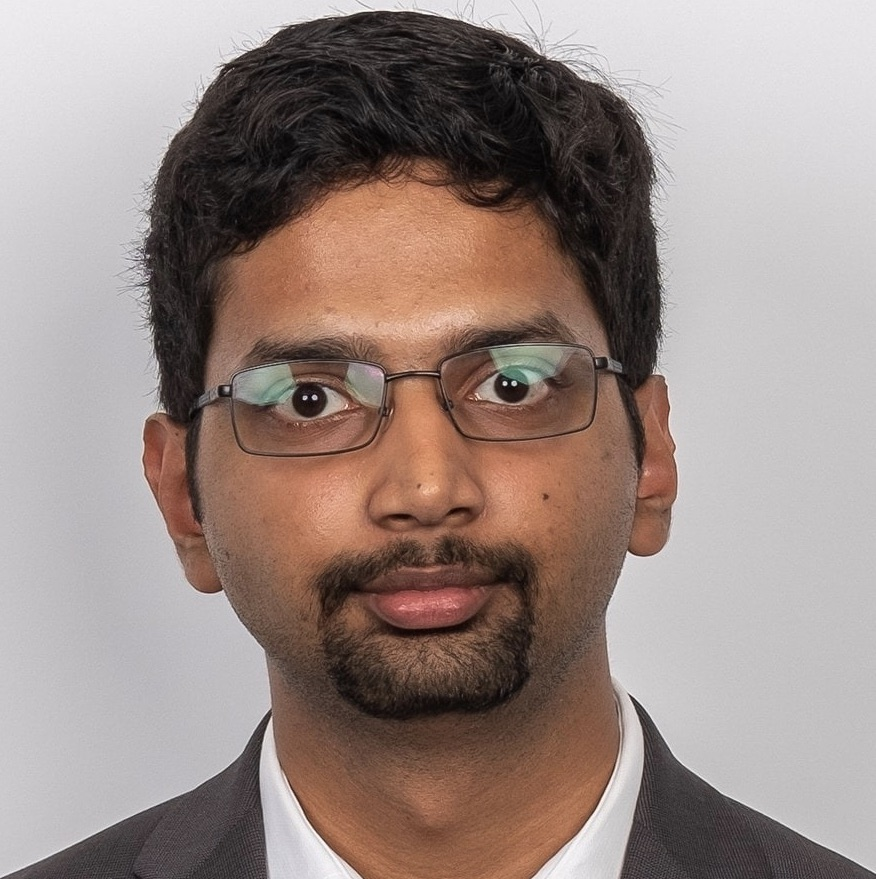
\includegraphics[width=.9in,clip,keepaspectratio]{tim/rahul.jpeg}}] {Rahul Yedida} is a PhD student in Computer Science at NC State University. His research interests include automated software engineering and machine learning for software engineering.   \url{https://ryedida.me}.
\end{IEEEbiography}
\vspace{-20mm}
\begin{IEEEbiography}[{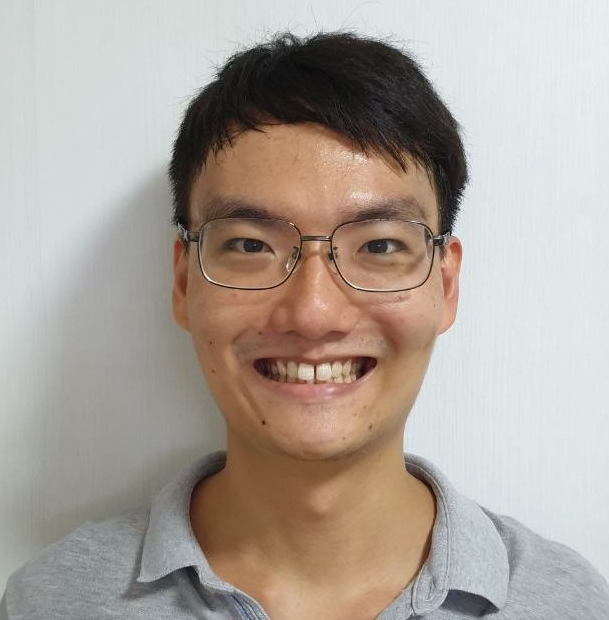
\includegraphics[width=.9in,clip,keepaspectratio]{tim/hongjin.jpg.png}}]{Hong Jin Kang  } is a Ph.D. student at Singapore Management University. His research interests include machine learning for software engineering, and mining rules and specifications.
 \url{https://kanghj.github.io/}.
\end{IEEEbiography}
\vspace{-20mm}
\begin{IEEEbiography}[{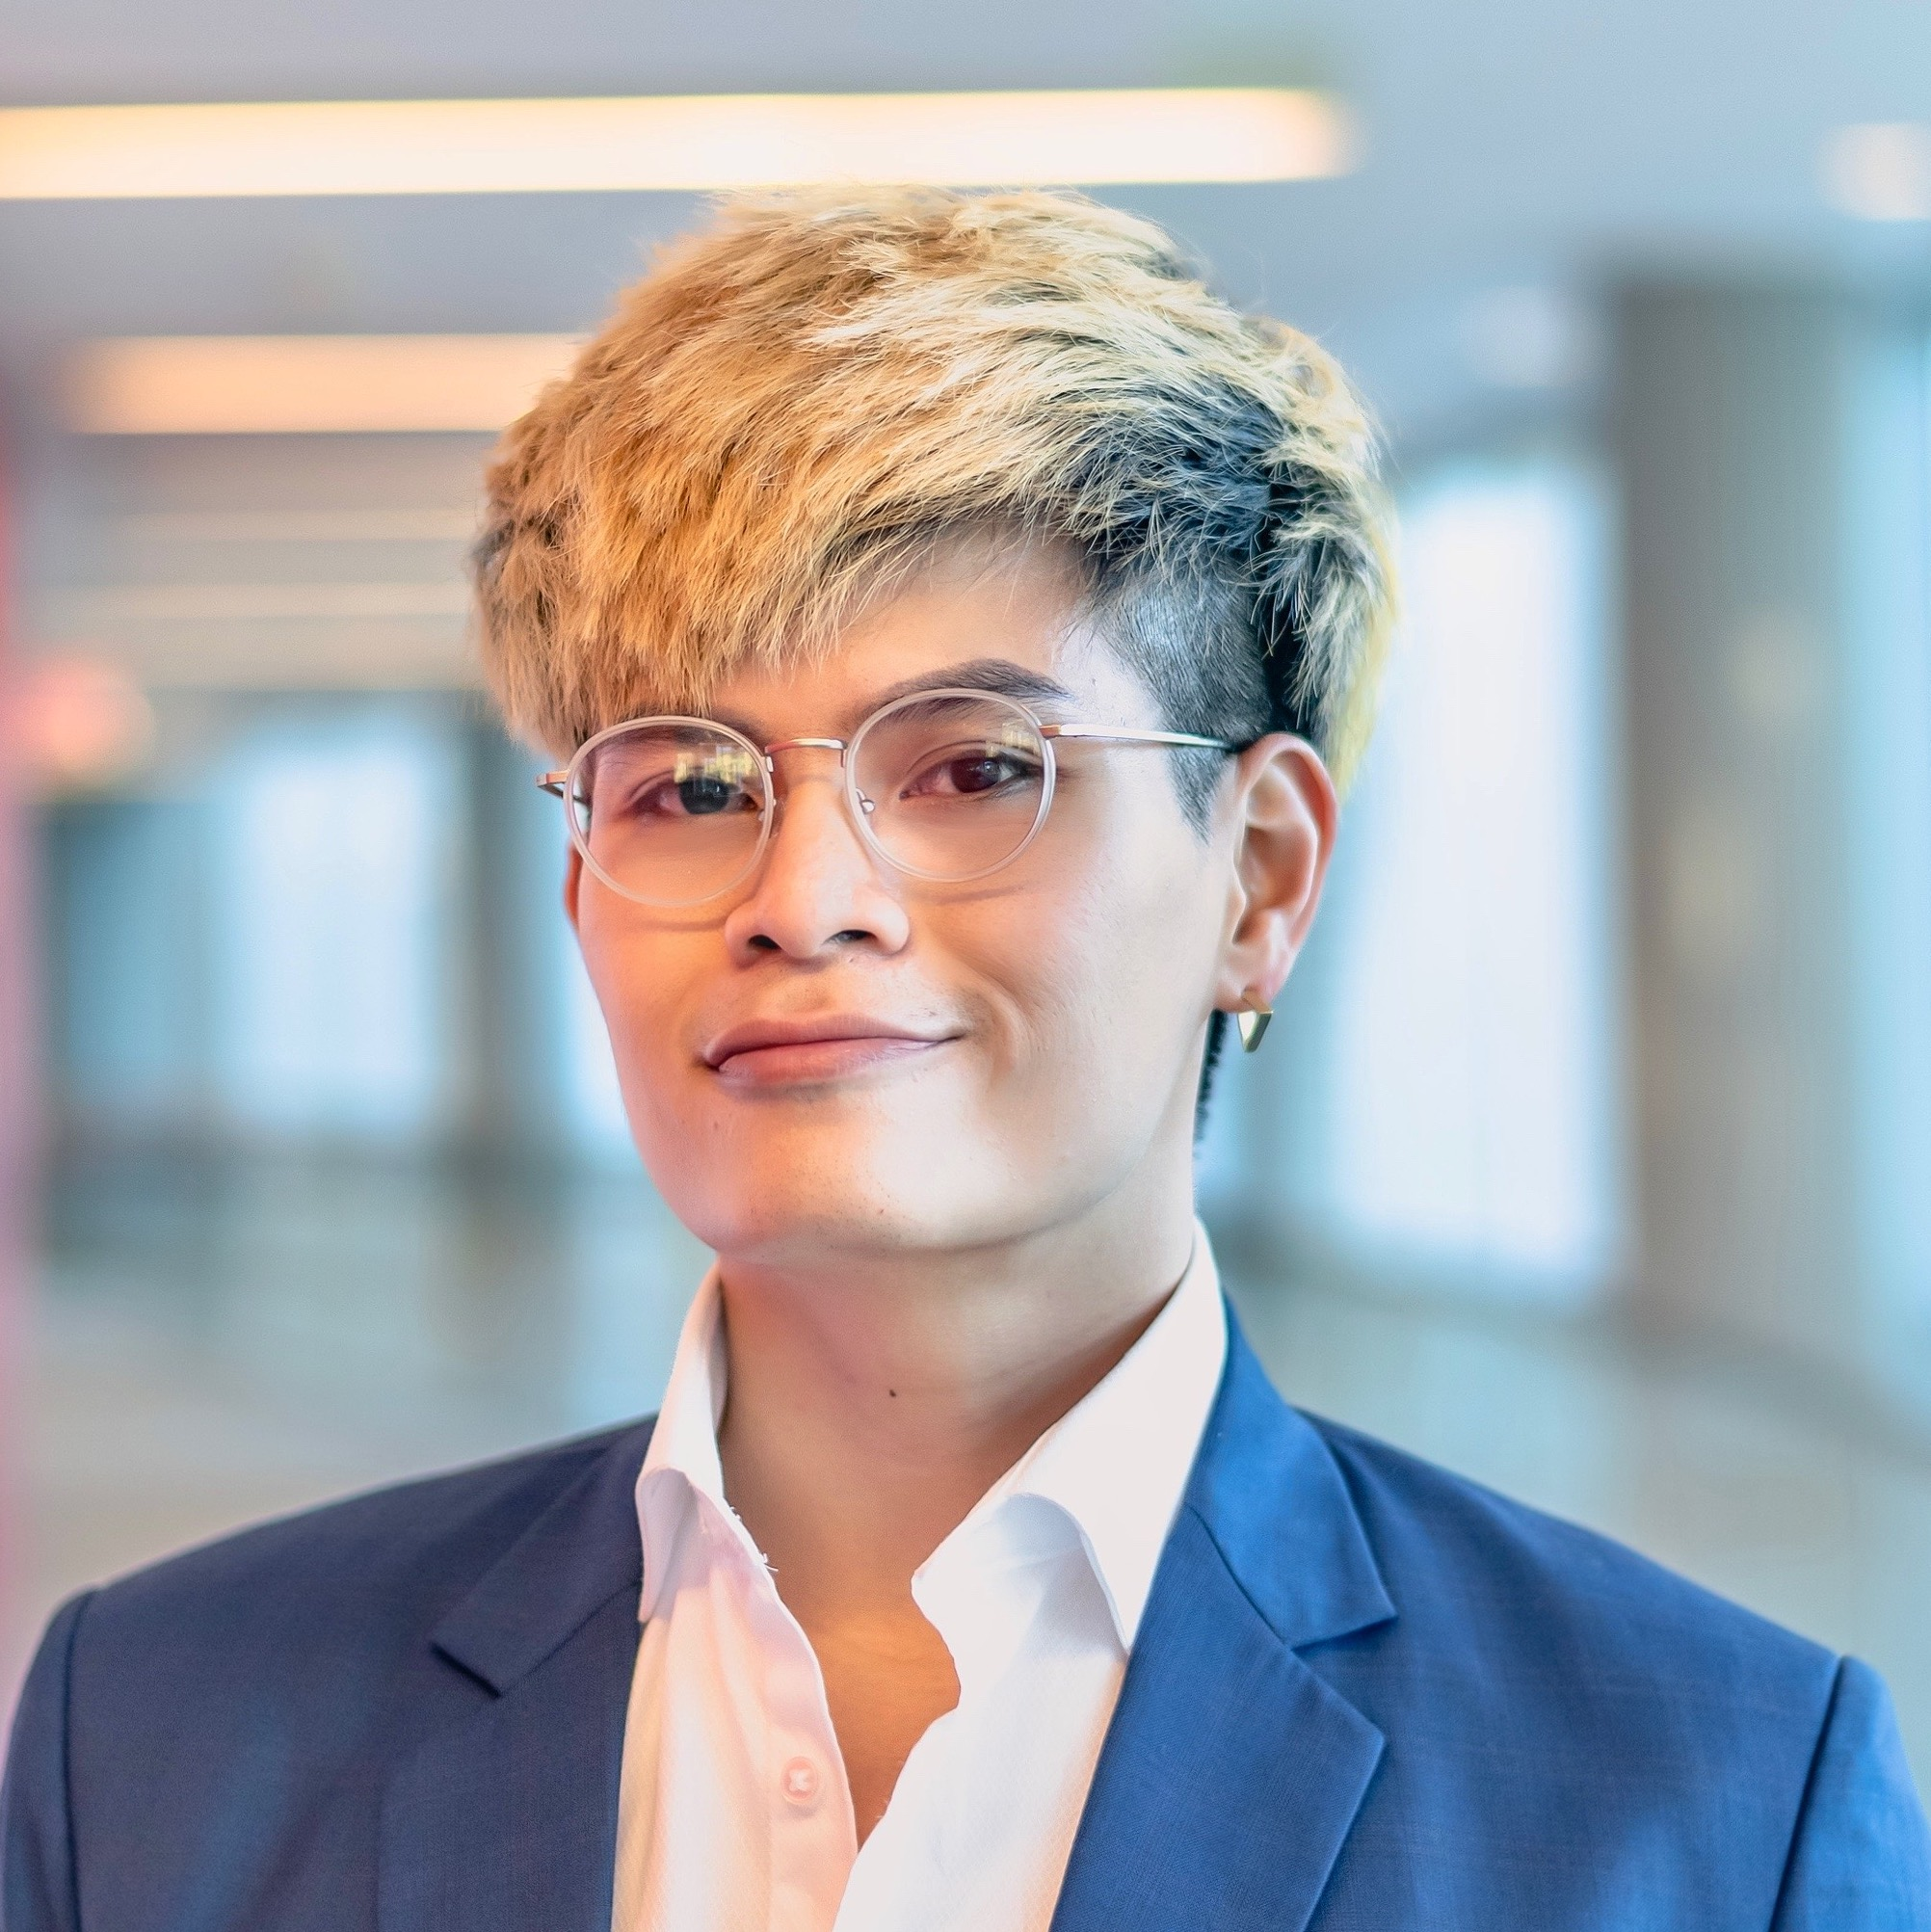
\includegraphics[width=.9in,clip,keepaspectratio]{tim/KT.JPG}}]{Huy Tu} holds a Ph.D. in Computer Science from North
Carolina State University, Raleigh, NC. They explored frugal labeling 
processes while improving the data quality for software analytics. Now, they works for Meta Platforms, Inc.  \newline \url{https://kentu.us}.
\end{IEEEbiography}
\vspace{-20mm}
\begin{IEEEbiography}[{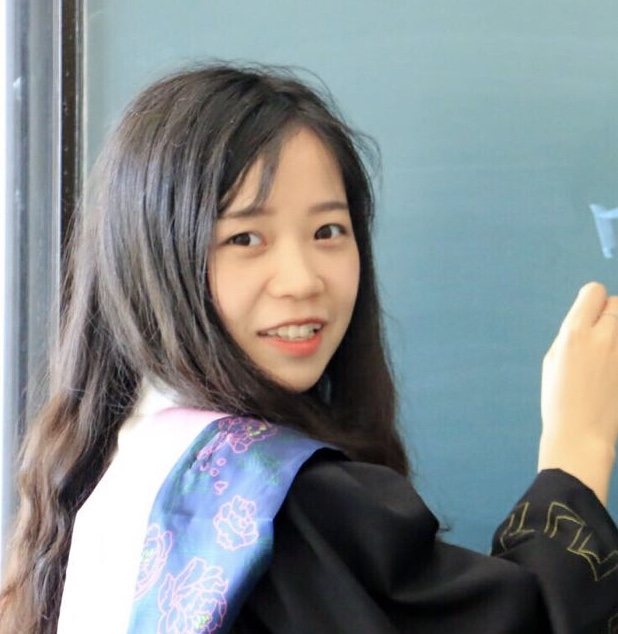
\includegraphics[width=.9in,clip,keepaspectratio]{tim/sherry.png}}]{Xueqi Yang} is a Ph.D. student in Computer Science at North Carolina State University.  Her research interests include automatic static analysis and applying human-assisted AI algorithms in software engineering.  \url{https://xueqiyang.github.io/}.
\end{IEEEbiography}
\vspace{-20mm}
\begin{IEEEbiography}[{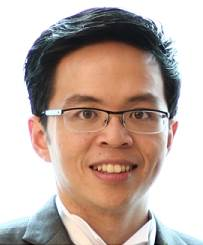
\includegraphics[width=.8in,clip,keepaspectratio]{tim/davidlo.jpg}}]{David Lo} is a Professor in Computer Science at Singapore Management University. His research interests include software analytics, empirical software engineering, cybersecurity, and SE4AI.   \url{http://www.mysmu.edu/faculty/davidlo/}.
\end{IEEEbiography}
\vspace{-20mm}
\begin{IEEEbiography}[{
\includegraphics[width=.9in,clip,keepaspectratio]{tim/menzies.png}}]{Tim Menzies} (IEEE Fellow, Ph.D. UNSW, 1995)
is a Professor in computer science  at NC State University, USA.
His research interests include software engineering (SE), data mining, artificial intelligence, and search-based SE, open access science.  \url{http://menzies.us}.
\end{IEEEbiography}
 
% %%%%%%%%%%%%%%%%%%%%%%%%%%%%%%
% % REVIEWER RESPONSES ROUND 1 %
% %%%%%%%%%%%%%%%%%%%%%%%%%%%%%%
\clearpage

\setcounter{page}{1}
\pagenumbering{roman}
\normalsize
\twocolumn
\newpage
% \twocolumn
%\linenumbers
\section*{Response to Reviewers}
\subsection*{Response to AE}

\begin{formal}
Dear authors, as you will see the reviewers have now commented on your manuscript.  All 3 reviewers think this is a highly relevant paper for TSE, but they also have concerns with regard to the methodology and the depth of explanation in the paper. I hope that the feedback can help you make improvements in these areas.
\end{formal}

Thank you for this opportunity to revise this paper. We wish to thank the reviewers for their careful and insightful comments. Our revisions are marked as \respto{2a(1-3)} and \respto{3a(1-3)} respectively. All changed text is highlighted in \textcolor{blue}{blue}.

Also, we have a question for you. We \underline{thought} that Figure1 was
useful to set the scene. Now reviewer1 says otherwise so perhaps we failed
in that regard. But please, what is your view? Delete figure1?

\subsection{Response to Reviewer 1}

\begin{formal}
The topic is interesting, since indeed static analyzers tend to list enormous amounts of suggestions, which are not manageable by software engineers. On top of that, methodologically, the paper is great, and to my understanding (though not an expert on machine learning) very sound.
\end{formal}

\begin{response}{1a1}
Thank you for your kind words. Much appreciated!
\end{response}

\begin{formal}
However, as a person oriented to the practical benefits of software engineering research, the paper has left me with a huge gap on what a practitioner can learn from this work. I agree that the paper can be of interest to researchers, since it presents a very interesting and novel methodology, but unfortunately there is not practical implication at all.
\end{formal}

\begin{draftresponse}{1a2}
Timm to Rahul: extract business case from odler apers. Make 2.1 another half page long Should we say that this tool could be incorporated into commercial applications such as IDEs, and be used as a filter step before warnings are shown to developers?
\end{draftresponse}

\begin{formal}
Additionally, the paper stays at a very high-level, treating the models as complete black-boxes, not giving any indication on which parameters of the warnings can consist them actionable.
\end{formal}

\begin{draftresponse}{1a3}
\begin{itemize}
    \item LIME (Sherry)
    \item \url{https://stats.stackexchange.com/a/261012/212844} (Rahul)
\end{itemize}
\end{draftresponse}

\begin{formal}
the paper’s title is a bit overselling: As far as I can understand, the dataset comes solely from FindBugs. Although I agree that FindBugs is a tool that deserves investigation, the results cannot be generalized to all static analyzers.  Also, not all static analyzers are there for finding “bugs”, for instance Sonar is a static analyzer for finding maintainability problems, or PMD for security problems, CheckStyle for style conventions, etc.
\end{formal}

\begin{response}{1a4}
We agree! We have modified our paper title to indicate that our work is specifically related to the FindBugs tool.
\end{response}

\begin{formal}
Figure 1 is not necessary, since a screenshot from FindBugs outputs does not provide any clear benefit for the readability nor the motivation
\end{formal}

\begin{response}{1a5}
Thank you for your feedback.  We had thought that the figure make it clear
to absolute beginners in this field what is going on.  If you are adamant in the regard, please say so and we will of course  delete it.
\end{response}

\begin{formal}
References used to support your claim on the lack of actionable outcomes from SAs are quite old, about 15 years ago. Maybe the situation has changed? Please update
\end{formal}

\begin{draftresponse}{1a6}
Sherry
\end{draftresponse}

\begin{formal}
The term ``actionable'' might not be correct. Something that is actionable, means that you can do something with this suggestion, giving motivation to do something is a bit different
\end{formal}

\begin{draftresponse}{1a7}
That's a fair point! We used ``actionable'' to mean, ``\textit{capable} of being acted on'' (Merriam-Webster's definition), to imply that these are static warnings that are less likely to be ignored by developers, for various reasons. We found it difficult to encapsulate the various reasons for ignoring static code warnings in one word.
\end{draftresponse}

\begin{formal}
``…showed that: (a)….'' There is no (b)
\end{formal}

\begin{response}{1a8}
Thank you for pointing that out! We have fixed that issue now.
\end{response}

\begin{formal}
The motivation that past work of the two groups was faulty, the published results were not correct, a new paper comes to solve the problem is a bit strange… How do you know what the new data extraction is correct? In later stages you refer to 2 human evaluators that disagreed with the original characterization. To me the level of evidence to characterize a published past study as not useful is not strong. What if the 2 evaluators had a biased mindset? The two evaluators were the authors of [25] and of this work. After reading [25] I found only one sentence explaining the process of tagging the warnings. What is the industrial experience of these two authors so as to be considered as “golden set”? I am extremely skeptical on this. Since the “faulty” research that needs to be revised (since the results were not correct) partially belongs to the authors of this work, what is your plan for that?  Are you planning to contact EMSE and ESWA editors?
\end{formal}

\begin{response}{1a9}
The labeling of the warnings were done with consideration of both the source code that the warnings were reported on as well as the subsequent evolution of the source code based on the projects’ revision control history. This provides a large amount of context to be analyzed by the annotators. One annotator was an undergraduate student while the other had 2 years of industrial experience. The annotators achieved strong inter-annotator agreement (Cohen’s Kappa $>$ 0.8) when labeling the warnings independently, which suggests that using the additional context of the revision control history led to high quality labels. We will provide more details of the construction of the dataset. 

We add the following information regarding the construction of the dataset in Section 5.1 (Data) with modifications in yellow:

\begin{blockquote}
{Recall that Kang et al. manually labelled warnings from the same projects studied by Yang et al. [54] to assess the level of agreement between human annotators and the heuristic. The manual labelling was performed by two human annotators. \hl{One annotator is an undergraduate student, while the other is a graduate student with two years of industrial experience.} When the annotators disagreed on the label of a warning, they discussed the disagreement to reach a consensus. While they achieved a high level of agreement, achieving a Cohen’s Kappa of above 0.8, manual labelling is costly, requiring human analysis of both the source code and the commit history of the code. That said, \hl{considering the subsequent evolution of the source code allows the annotators to analyze each warning with a greater amount of context.} These labels are essential since it removed closed warnings which are not actionable (e.g., the warnings may have been removed for reasons unrelated to the Findbugs warning)}
\end{blockquote}

While the findings of the prior studies have to be weakened, there are still important insights that are relevant to both researchers and practitioners. To aid the discovery of this paper which builds on the prior studies, we will add a note linking to this paper on the artifact websites of the previous papers.
\end{response}

\begin{formal}
Why shall a software engineer be interested in checking which data mining methods are recommended? This sound like very theoretical research question. A software engineer would care about which warnings she needs to consider. What are their common characteristics
\end{formal}

\begin{response}{1a10}
You raise an important point! Although our results have practical applications, we believe there is value in adding theoretic understanding to the SE (and more broadly, computer science) literature. There is value in studying not only the \textit{how} (i.e., how do we solve problem X), but also the \textit{why} (i.e., why does solution Y work). 

Indeed, if you look closely at our approach, the underlying learner is a feedforward learner; the GHOST approach that we rely on used the theoretical results of \citet{montufar2014number} to choose the range for hyper-parameter options. Therefore, while the question of which data miner is better might be a question that interests theorists more, we still find value in that contribution.
\end{response}

\begin{formal}
``For complex data, global….''. This is not understandable at all by a non-expert. What is a local treatment? What is a localized treatment? How do they map the current problem?
\end{formal}

\begin{response}{1a11}
Agreed! We have added more text discussing this before mentioning those terms \citeresp{1a11.1}.
\end{response}

\begin{formal}
I am surprised that there is no question on which predictors are the most important. I see a long list of treatments studied, but not any refence on what data these models run upon. Treating ML models as black-boxes does not help a lot in practice. In the end, what do we learn from this work, apart from the fact the accuracy of a GHOST2 model is better than any other model, for this specific dataset, for this specific problem, if the solution to the problem is not given. What are the actionable static analysis warnings?
\end{formal}

\begin{draftresponse}{1a12}
This will depend on LIME's results.
\end{draftresponse}

\begin{formal}
The writing the paper is excellent, the background on ML, statistics, data analysis is also excellent. The authors are real experts on that, and I believe that if they also try to shed light on some practical aspects of this problem, this can be an excellent paper.
\end{formal}

\begin{response}{1a13}
Thank you for the kind words!
\end{response}

\begin{formal}
In Section 5, I wonder: if I try 144 different treatments, in the end, wouldn’t always one be of great accuracy?
\end{formal}

\begin{response}{1a14}
Yes, by definition. In Section \ref{rigg} (which is where the 144 number is mentioned), we aimed to reduce the number of those 144 that we needed to run by a process of elimination (i.e., if treatment A does not help, then do not try treatments that use A). That was the basis for our ablation study, whose treatments are shown in Table \ref{tab:treatments}. 
\end{response}

\begin{formal}
Also, in Section 5, why are you ignoring completely the model. I would expect some presentation of how the model is built. What are the independent variables? How do you collect them? I only see how you calculate the dependent variable (if a warning is actionable)—see previous comment on this
\end{formal}

\begin{response}{1a15}
Agreed--we did not talk much about the model itself. This was because the actual model is encapsulated in DODGE, and is a feedforward learner whose hyper-parameters are chosen based on theoretical deep learning literature. We have now added more text describing this \citeresp{1a15.1}
\end{response}

\subsection{Response to Reviewer 2}

\begin{formal}
It also seems like the entire paper is focused on Kang’s dataset of static analysis bugs and how to fix mislabelling in that dataset. This paper is more about data engineering to clean data from the bad dataset before feeding it into machine learning models. The title of the paper must also be appropriate to that. They can try to show their results on one more erroneous dataset.
\end{formal}

\begin{response}{2a1}
We agree! Reviewer 1 also pointed out this issue with the paper title, and we have changed it now.
\end{response}

\begin{formal}
The ordering is somewhat random smote -> ghost -> ghost -> smote -> smooth -> dodge. Also, this ordering is inspired by a paper that already performs smote+ ghost repeatedly. The contribution of the paper seems to be a mere application of already existing techniques just for the case of data in warnings of static analysis tools.
\end{formal}

\begin{response}{2a2}

\end{response}

\end{document}


